\documentclass[a4paper, 11pt]{report}
\usepackage{algorithmeUTF8}
\usepackage{changepage}
\usepackage{etoolbox}
\usepackage{fancyhdr}
\usepackage{fancyvrb}
\usepackage[french]{babel}
\usepackage{graphicx}
\usepackage{listings}
\usepackage{pdfpages}
\usepackage[T1]{fontenc}
\usepackage[utf8]{inputenc}
\usepackage{url}
\usepackage{verbatim}
\usepackage{xcolor}
\usepackage{hyperref}

\begin{document}

% configuration du pied de page
\pagestyle{fancy}
\fancyhf{} % efface le style par défaut

\fancyhead{} 
\renewcommand{\headrulewidth}{0pt} 

% ajout du logo insa (en bas à droite)
\fancyfoot[R]{
\includegraphics[width=1.5cm]{imagesRapport/logoInsaRouen.jpg}} 
% ajout du numéro de page (en bas au centre)
\fancyfoot[C]{\thepage}

\setlength{\footskip}{20pt}

% correction du style de page des chapitres pour appliquer correctement le pied de page à chacun
\makeatletter
\patchcmd{\chapter}{\thispagestyle{plain}}{\thispagestyle{fancy}}{}{}
\makeatother

% modifie le package hyperref pour eviter les cadre de couleurs autours des hyperliens 
\hypersetup{pdfborder=0 0 0}

% page de garde
\begin{titlepage}

    \centering
    
\includegraphics[scale=0.3]{imagesRapport/logoInsaRouen.jpg}~\\[0.1cm]
    \textsc{\LARGE Institut National Des Sciences Appliquées}\\[0.1cm]
    \textsc{\LARGE ROUEN NORMANDIE}\\[0.5cm]
    \textsc{\Large Rapport de projet}\\[0.5cm]
    
    {\huge\bfseries Projet Integratif Smart Robot \par}
    \vspace{0.5cm}
   
    Étudiants:\\
    Yohann \textsc{Delaplace}\\
    Louis \textsc{Lenoble}\\
    Maël \textsc{Planchot}\\
    Dylan \textsc{Sanson}\\
    Nathan \textsc{Sourdrille}\\
    \vspace{0.5cm}
    
    Professeurs référents:\\
    $M^{me}$ \textsc{Laghmara}\\
    $M^{r}$ \textsc{Delestre}
    
    \vspace{2cm}
   
    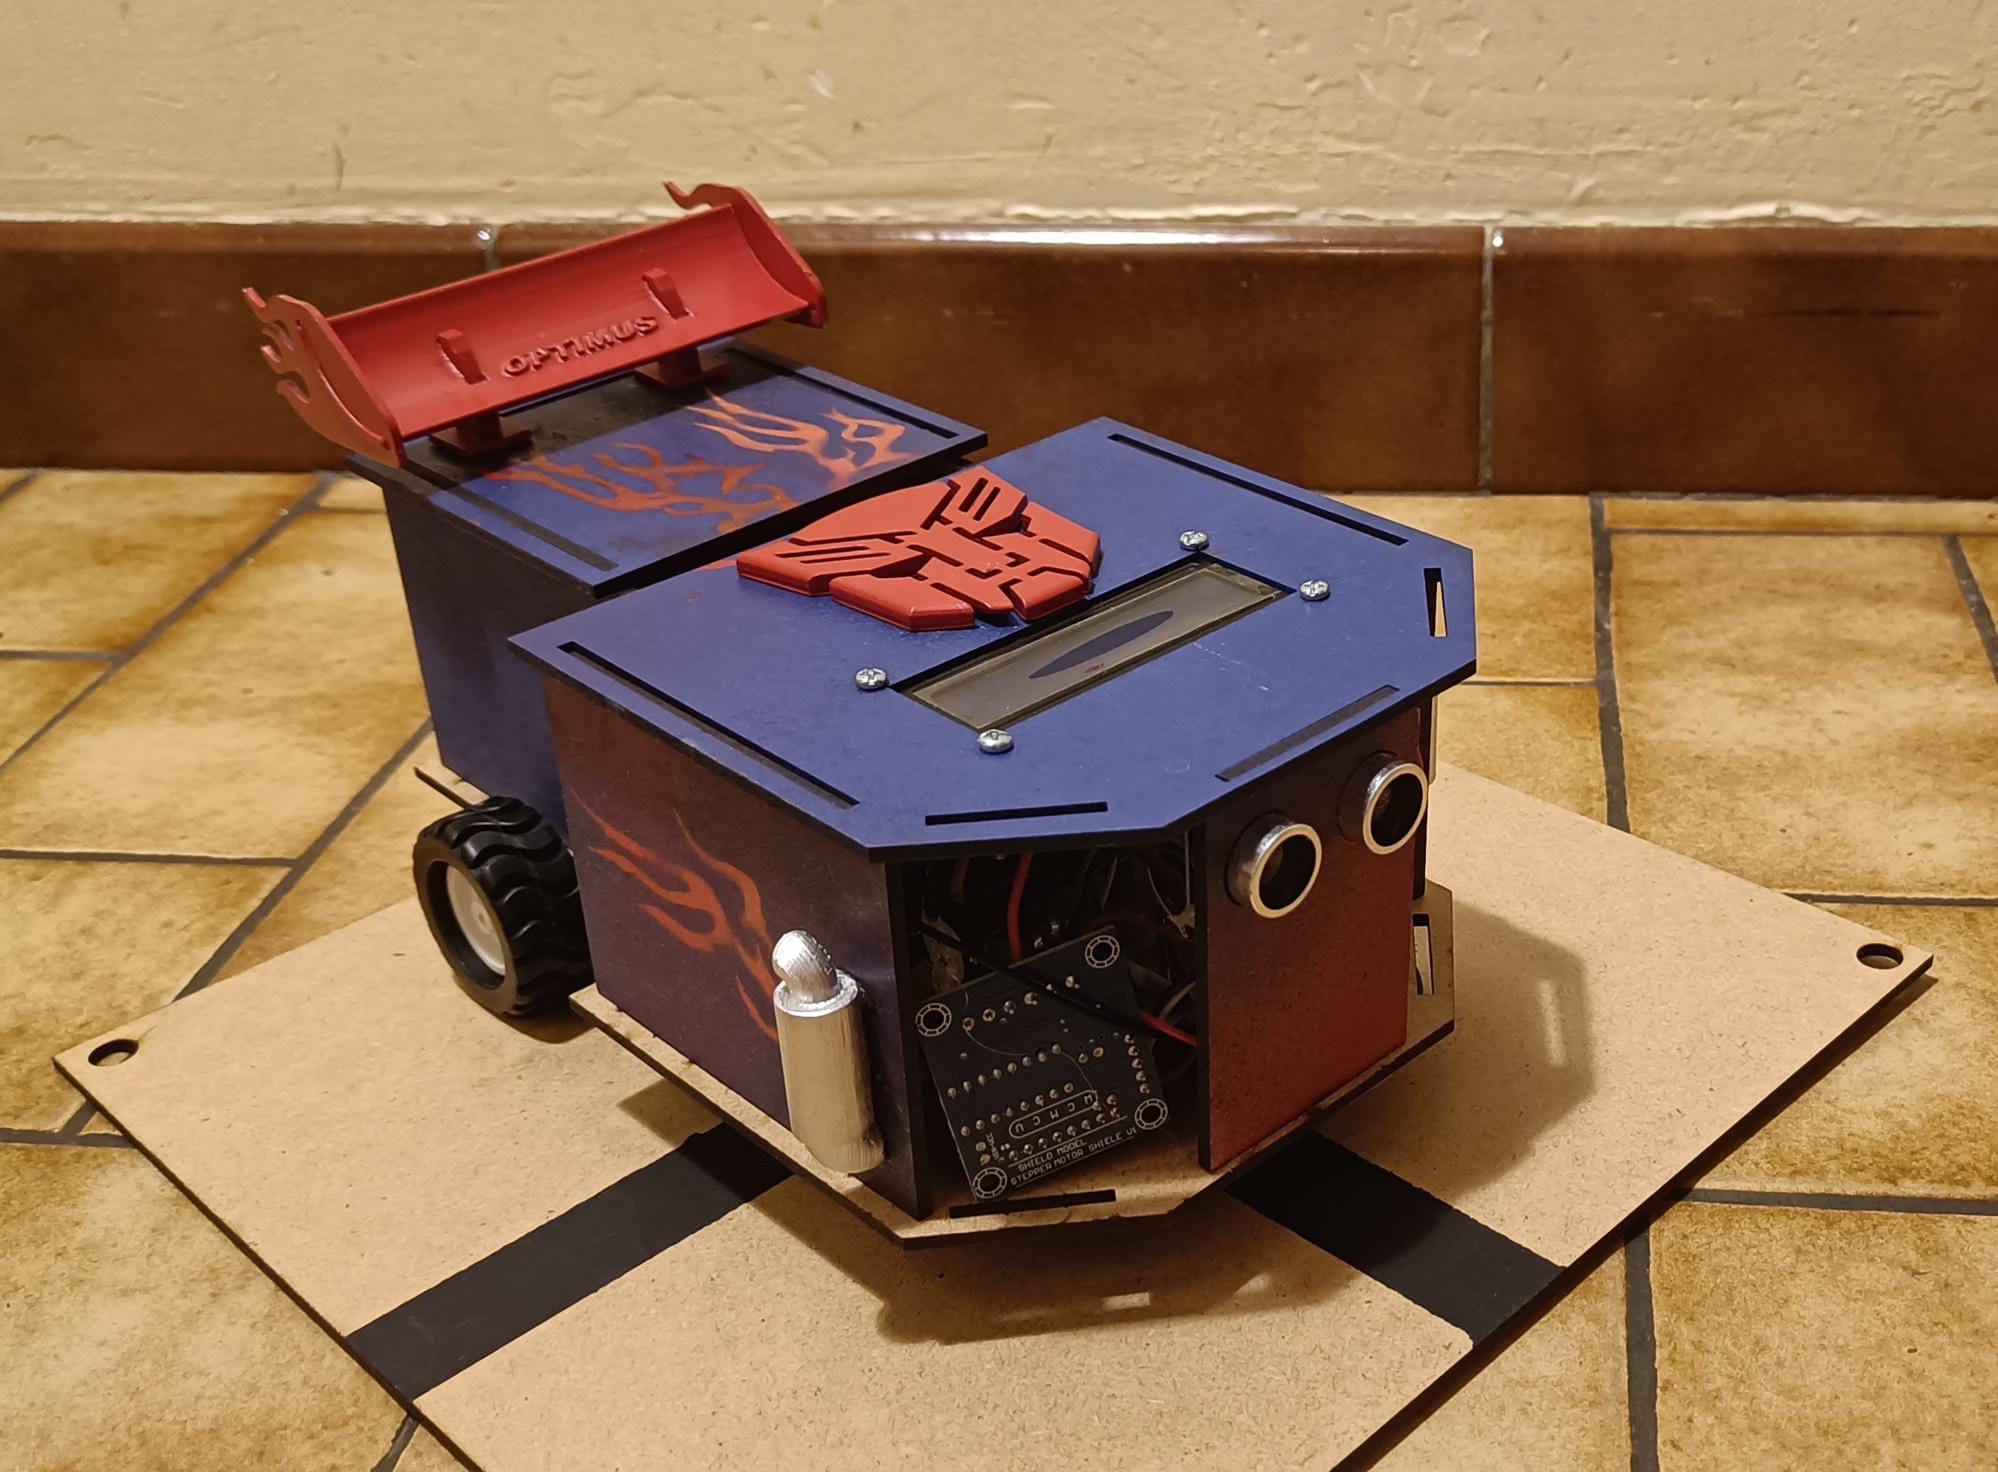
\includegraphics[width=0.5\textwidth]{imagesRapport/photoRobot.jpeg}\par

\end{titlepage}

\tableofcontents
\pagestyle{fancy}

% remerciements
\chapter{Remerciements}

Tout d'abord, nous tenons particulièrement à remercier les professeurs référents, \textbf{$M^{me}$ \textsc{Laghmara}}, \textbf{$M^{me}$ \textsc{Planterose}} ainsi que \textbf{$M^{r}$ \textsc{Delestre}} pour leur accompagnement et leur investissement tout au long du projet.
Nous tenons également à remercier l'ensemble des intervenants qui nous ont permis de poursuivre notre développement du robot et au département ITI pour tout le matériel mis à notre disposition.





% introdution
\chapter{Introduction}
\newcommand{\ordre}{\textbf{Ordre}}
\newcommand{\direction}{\textbf{Direction}}
\newcommand{\nnn}{\textbf{NaturelNonNul}}
\newcommand{\Labyrinthe}{\textbf{Labyrinthe}}
\newcommand{\cdc}{\textbf{ChaineDeCaracteres}}

Dans le cadre de nos études en troisième année à l'INSA Rouen Normandie au sein du département ITI, nous avons reçu l'opportunité de participer au projet Integratif Smart Robot. Celui-ci vise à renforcer et développer des compétences que nous avons abordé en cours. Notre objectif était de concevoir un robot capable de sortir le plus rapidement possible d’un Labyrinthe de forme carré, en suivant une ligne pour se guider.

\section{Différentes compétences}
Ce projet se compose notamment de deux grandes parties, celles-ci nécessitant des compétences en algorithmique et en électronique.
Nous nous sommes appuyés sur les outils suivants pour réaliser ce projet:
\begin{itemize}
    \item \texttt{Doxygen} pour la génération de la documentation du code.
    \item \texttt{Fritzing} pour la conception du circuit électronique.
    \item \texttt{GitLab} pour le partage du code source et la création de tickets des actions et demandes.
    \item \texttt{Make} pour la compilation du code source.
    \item \texttt{LaTeX} pour générer un rapport de projet en .pdf après compilation.
\end{itemize}
\subsection{Algorithmique}
Tout d'abord, la partie algorithmique permet de créer un algorithme et de l'implémenter permettant de trouver le chemin le plus court pour sortir du labyrinthe. Cette implémentation est le résultat de différentes étapes du cycle en V, celles-ci sont détaillés dans la suite du rapport.
\subsection{Électronique}
La partie électronique a pour but de concevoir le robot qui va utiliser l'algorithme pour sortir du labyrinthe. Ainsi, cela nous a poussé à la réflexion du placement des différents composants sur le robot. Cette conception a fait appel à différentes compétences, comme la création d'un schéma électronique et son câblage associé, le codage sur carte Raspberry, la soudure ...
\vspace{5mm}

\section{Organisation du travail}

L'outil GitLab permet le partage du code dans le groupe mais propose également la création de tickets pour suivre les modifications. Ainsi, nous avons créé les tickets suivants afin d'effectuer les tâches requises par le projet. Chaque ticket sera référencé par un \# suivit de son numéro (le numéro suit l'ordre de création des tickets): 
\vspace{2mm}

\begin{itemize}
    \item \#2: ce qui concerne latex.
    \item \#3: ce qui concerne les TADs.
    \item \#4: ce qui concerne l'analyse descendante (partie algorithmique/\\ électronique).
    \item \#5: ce qui concerne le schéma électrique et le fritzing.
    \item \#6: ce qui concerne la conception préliminaire et la conception détaillée.
    \item \#7: ce qui concerne la fonction creerLabyrinthe.c.
    \item \#8: ce qui concerne la fonction analyseFichier.c.
    \item \#9: ce qui concerne la fonction resolutionLabyrinthe.c.
    \item \#10: ce qui concerne le code du robot.
    \item \#11: ce qui concerne tous les types.c.
    \item \#12: ce qui concerne les tests unitaires.
    \item \#13: ce qui concerne les makefiles.
    \item \#14: ce qui concerne l'espace de nommage.
    \item \#16: ce qui concerne la documentation de la partie électronique.
    \item \#17: ce qui concerne les tests sur le robot.
    \item \#18: ce qui concerne le script bash.
\end{itemize}
\vspace{5mm}

Les tickets étaient ainsi à disposition de chaque membre du groupe afin d'assurer la bonne organisation du projet et le suivi des tâches. Cependant, pour assurer le bon déroulement du projet, la répartition du travail était indiqué par le chef de projet. Ainsi, chaque membre du groupe s'est vu attribuer différentes tâches tout au long du projet. En cela, chaque membre du groupe a pu travailler sur différents aspects du projet:

\begin{itemize}
    \item \textbf{Delaplace Yohann}\\
    développement des makefile, bash et tests unitaires,\\
    rédaction du rapport latex.
    \item \textbf{Lenoble Louis (chef de projet)}\\
    organisation du projet,\\
    montage du robot,\\
    développement de la partie algorithmique.
    \item \textbf{Planchot Maël}\\
    développement de la partie électronique et Doxygen.
    \item \textbf{Sanson Dylan}\\
    développement de la partie algorithimique et électronique.
    \item \textbf{Sourdrille Nathan}\\
    développement de la partie algorithmique et électronique,\\
    rédaction du rapport latex et bilan de chaque séance.
    
\end{itemize} 
\vspace{0.5cm}

\textbf{Planning :}\\
Afin de maintenir un bon rythme de travail et de pouvoir mener le projet à son terme, nous avons mis en place un planning qui respecte les critères suivants: 
\begin{itemize}
\item {Les tâches à faire avant la séance}
\item {Les tâches à faire durant la séance}
\item {Le déroulement de la séance}
\item {Le bilan de fin de séance}
\end{itemize} 
\vspace{0.5cm}
Voici, par exemple, le planning concernant les séances d'électronique :

\begin{figure}[h!]
    \hspace{-2cm}
    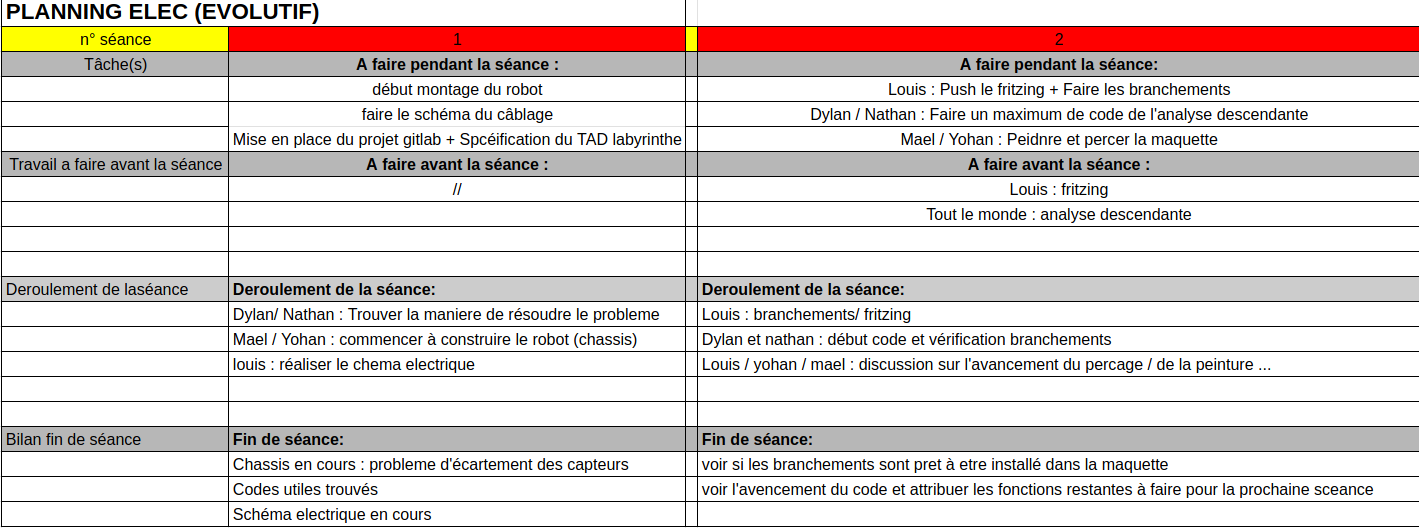
\includegraphics[width=1.2\textwidth]{imagesRapport/planning1.png}
    \caption{planning séances 1 et 2}
    \label{fig:exemple}
\end{figure}
\begin{figure}[h!]
    \hspace{-2cm}
    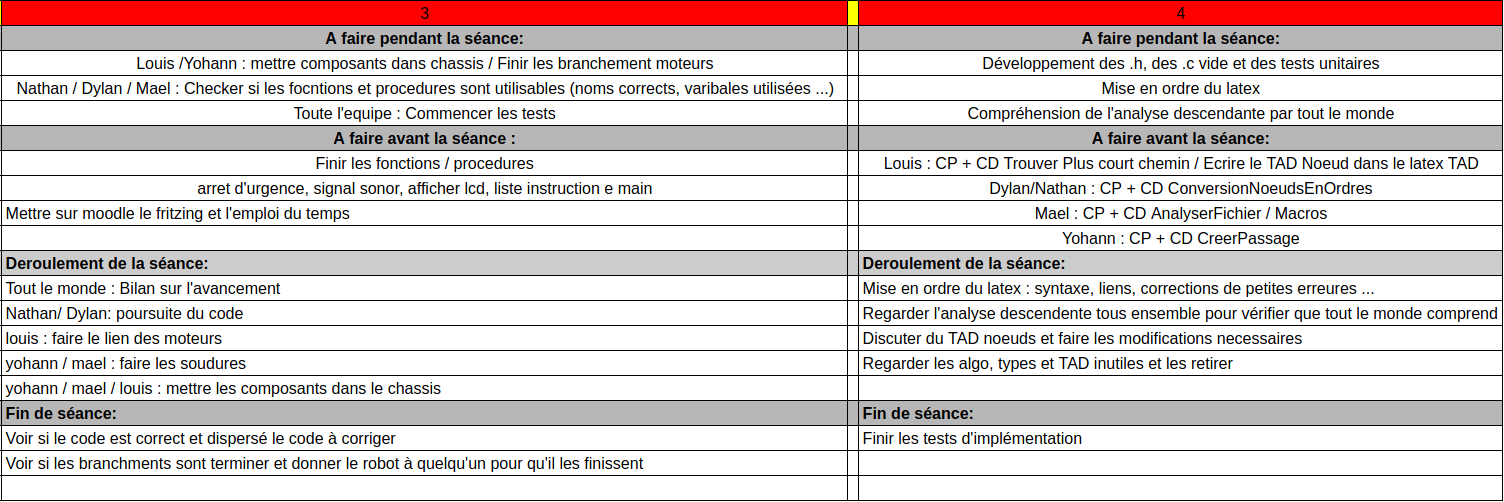
\includegraphics[width=1.2\textwidth]{imagesRapport/planning2.png}
    \caption{planning séances 3 et 4}
    \label{fig:exemple}
\end{figure}
\vspace{5cm}

\textbf{Matrice des tâches réalisées}\\
Afin de mieux visualiser l'implication de chaque membre du groupe dans les différentes étapes du projet, ci-dessous est présenté la matrice des tâches réalisées (le niveau d'implication dans chaque tâche est indiqué via un pourcentage) :
\begin{table}[ht]
\begin{adjustwidth}{-3cm}{-3cm}
\centering
\begin{tabular}{|p{2.2cm}|p{2.2cm}|p{2.2cm}|p{2.2cm}|p{2.2cm}|p{2.2cm}|}
\hline
\textbf{Tâches} & \textbf{Delaplace Yohann} & \textbf{Lenoble Louis} & \textbf{Planchot Maël} & \textbf{Sanson Dylan} & \textbf{Sourdrille Nathan} \\
\hline
schéma électronique fritzing & 0 & 100 & 0 & 0 & 0 \\
\hline
choix du placement des capteurs & 20 & 20 & 20 & 20 & 20 \\
\hline
création des TAD & 20 & 20 & 20 & 20 & 20 \\
\hline
analyse descedante & 20 & 20 & 20 & 20 & 20 \\
\hline
recherche algorithme de résolution & 0 & 33 & 33 & 33 & 0 \\
\hline
conception détaillée des fonctions principales & 0 & 33 & 33 & 33 & 0 \\
\hline
développement des .h (algo) & 0 & 65 & 0 & 25 & 10 \\
\hline
développement des .h (élec) & 0 & 0 & 50 & 50 & 0 \\
\hline
développement des .c (types) & 0 & 50 & 0 & 20 & 30 \\
\hline
développement des .c (algo) & 20 & 40 & 0 & 40 & 0 \\
\hline
développement des .c (élec) & 0 & 0 & 60 & 30 & 10 \\
\hline
tests unitaires (algo) & 90 & 0 & 0 & 5 & 5 \\
\hline
tests unitaires (élec) & 20 & 20 & 20 & 20 & 20 \\
\hline
tests d'intégration (algo) & 0 & 50 & 0 & 50 & 0 \\
\hline
tests d'intégration (élec) & 20 & 10 & 50 & 10 & 10 \\
\hline
makefile & 90 & 0 & 10 & 0 & 0 \\
\hline
bash & 100 & 0 & 0 & 0 & 0 \\
\hline
mise en place de doxygen & 0 & 0 & 100 & 0 & 0 \\
\hline
documentation & 0 & 33 & 33 & 33 & 0 \\
\hline
mise en place du latex & 50 & 0 & 50 & 0 & 0 \\
\hline
rapport latex & 25 & 5 & 0 & 0 & 70 \\
\hline

\end{tabular}
\end{adjustwidth}
\end{table}

 

% Partie életronique
\chapter{Partie électronique : schéma électrique}

La toute première étape du projet a été de choisir les composants que nous allions utiliser, leur emplacement sur le robot ainsi que leur branchement. Bien que ce soit une étape qui peu paraître plutôt simple, celle-ci joue un rôle clé dans la préparation du projet. En effet, il faut réussir à s'accorder  sur la manière dont va fonctionner le robot pour que chacun puisse travailler de manière autonome. De plus, elle permet d'anticiper l'élaboration de l'analyse descendante.\\

Ci-dessous sont présentés le schéma électronique mis en place, la liste des composants, ainsi que le bilan énergétique de ceux-là.
\vspace{0.5cm}

\textbf{Schéma électronique du robot}

\includepdf[pages=-, pagecommand={
    \thispagestyle{fancy} 
    \fancyhf{} 
    \fancyfoot[R]{\includegraphics[width=1.5cm]{logoInsaRouen.jpg}} 
    \fancyfoot[C]{\thepage} 
    \setlength{\footskip}{20pt}  
}]{elec/Schema_montage_Groupe_4.pdf}

      
\section{Explication du fonctionnement des différents composants}
    \subsection{Liste des différents composants utilisés}
    La carte Raspberry est reliée à différents composants ci dessous :    
	    \begin{itemize}
            \item $\bullet$ \textbf{1 capteur à ultrason} (situé sur le devant du robot) permet de détecter les potentiels obstacles se plaçant devant le robot.
            \item $\bullet$ \textbf{4 capteurs suiveurs de ligne} permettent au robot de suivre la ligne noir en la détectant continuellement. Concernant le placement des capteurs, il y en a 3 à l'avant (1 au centre, 1 à gauche, 1 à droite) et 1 à l'arrière (centré avec le capteur placé à l'avant au centre).
            \item $\bullet$ \textbf{2 moteurs} (situés à l'arrière) permettent au robot de se déplacer.
            \item $\bullet$ \textbf{1 carte moteur  } permet le contrôle des moteurs.  
            \item $\bullet$ \textbf{1 écran LCD} (situé sur le dessus du robot) permet l'affichage des commandes du robot en cours d'exécution.
            \item $\bullet$ \textbf{1 buzzer} (situé à l'arrière du robot) permet d'émettre un son lors de l'arrêt d'urgence.
            \item $\bullet$ \textbf{1 batterie } permet d'alimenter en électricité la carte Raspberry.
            \item $\bullet$ \textbf{2 piles } permettent d'alimenter les moteurs en électricité.
            \item $\bullet$ \textbf{1 bouton } (situé à l'arrière du robot) permet d'ouvrir ou fermer le circuit électrique et ainsi démarrer les moteurs.
            \item $\bullet$ \textbf{1 LED } (situé à l'arrière du robot) permet d'indiquer l'état de charge de la batterie.
        \end{itemize} 
    \vspace{5mm}
     
    \subsection{Capteur à ultrason} 

        Le capteur à ultrason envoie un signal sonore à l'aide d'un émetteur, puis le signal émis va percuter un obstacle et ainsi être réfléchi. Un capteur a ultrason faisant partie du dispositif va permettre de récupérer le signal réfléchi. Ainsi pour évaluer la distance entre l'objet et le capteur il suffit d'appliquer la formule suivante : \\ \\$\frac{360 \times temps \times V_{son}}{2} = distance$ \\ \\Le temps (en seconde) et la distance (en mètre) et $V_{son}$ la vitesse du son dans l'air (344m/s), permettent de déterminer à quelle distance se situe l'objet. Il ne reste ensuite plus qu'à programmer à partir de quelle distance minimale le robot doit s'arrêter. La distance minimale retenue est de 15cm.


    \subsection{Capteurs de ligne} 

        Les capteurs de ligne permettent de détecter une ligne sombre sur un fond clair et inversement. Les capteurs sont calibrés grâce à un potentiomètre situé sur le capteur. Ces capteurs possèdent 2 modes de sorties:
        
        \begin{itemize}
            \item Un mode de sortie analogique: plus la ligne est foncée, plus la valeur renvoyée est grande.
            \item Un mode de sortie tout ou rien: si la couleur du fond est supérieure au seuil défini par le potentiomètre alors le capteur renvoie 1, sinon il renvoie 0.
        \end{itemize} 
        \vspace{5mm}
        \ \ \ Dans notre cas, nous avons utilisé le mode tout ou rien pour détecter une ligne. 

    \subsection{Bouton on/off}
    
        Le bouton on/off (activation manuelle) est branché en série sur le circuit, il sert d'interrupteur afin de ne pas alimenter les moteurs lorsque le robot n'est pas en fonctionnement. Cela permet d'économiser de la batterie. 

    \subsection{LED}

        La LED s'allume quand la valeur du courant qui circule à l'interieur est supérieure à un certain seuil défini en fonction de la couleur de la LED. Dans notre cas la LED est rouge donc elle nécessite une tension comprise entre 1.8V et 2.1V pour s'allumer. Au dessus de cette limite, la led cesse de fonctionner et devient inutilisable. En dessous de cette limite, la LED ne s'allume pas (ou très peu) car elle agit comme une diode. 

    \subsection{Carte moteur}

        La carte moteur permet de contrôler les moteurs. Elle prend en entrée une alimentation externe et une tension définit par la formule suivante: \\ \\ $\frac{1024 \times vitesseMoteur}{100}$ \\ \\ La vitesse du moteur est en pourcentage (de 0 à 100) de la vitesse maximale du moteur. La carte moteur renvoie en sortie une tension et un courant adapté pour le moteur selon ses entrées. Ainsi grâce à cette formule, nous sommes capables de définir la vitesse de rotation du moteur, mais aussi d'activer ou de désactiver un moteur afin de réaliser un virage par exemple.
        
    \subsection{Buzzer}

        Le buzzer émet un signal sonore lorsqu'il reçoit une tension en entrée de 3.3V. 

    \subsection{Ecran LCD}

        L'écran LCD possède différents pixels qu'il faut mettre à jour afin d'afficher le contenu voulu. Pour le mettre à jour, on utilise les ports SDA et SCL de l'écran pour communiquer avec la carte Raspberry. Dans notre cas, l'écran LCD affichera les ordres en cours et la détection d'intersection. 
    
    \subsection{La carte Raspberry}

        C'est la carte électronique principale du robot ayant un OS intégré (linux). Elle est capable d'éxécuter des lignes de codes grâce à une barette de RAM et un processeur intégré. Elle possède en entrée des GPIOs qui permettent de contrôler des éléments externes comme le buzzer ou la carte moteur. Elle est alimentée via un câble USB-C et possède des ports pour brancher un écran, un clavier, une souris ... Une carte réseau est également intégrée, ce qui permet de contrôler la carte à distance via le protocole SSH. Le stockage est assérée via une carte micro-SD. 
        
        \textbf{Ci-dessous une vision simple du robot, pour comprendre sa structure globale}
        \begin{figure}[!h]
            \center 
            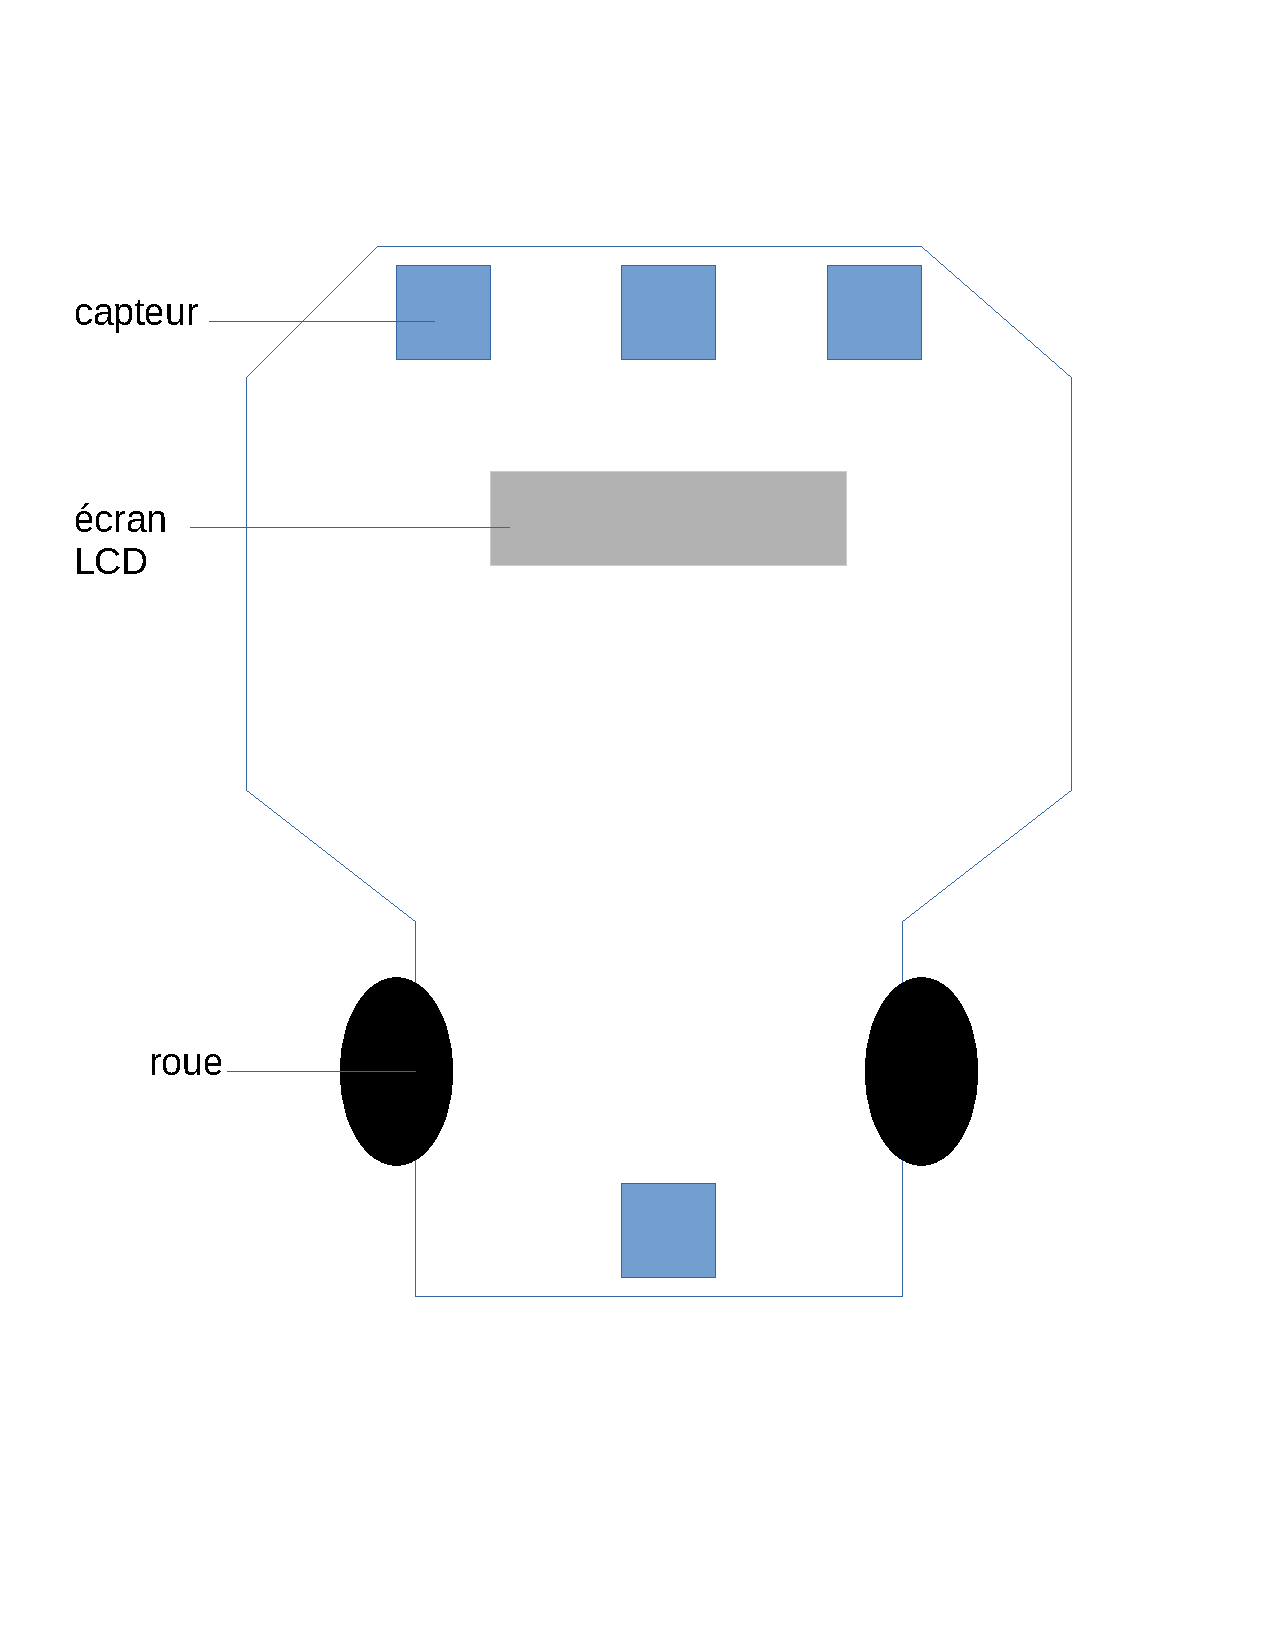
\includegraphics[width=0.9\linewidth]{imagesRapport/schema_simplifie_robot.pdf} 
            \caption{Schéma simplifié du robot}  
            \label{fig:analyse}
        \end{figure}
    
    
         
\newpage
\section{Explication du câblage}
 
La batterie est reliée à la carte Raspberry pour l'alimenter en électricité, ce qui permet à celle-ci d'exécuter le programme permettant le déplacement du robot.
De plus, la carte Raspberry est reliée, via les GPIOs, aux différents composants afin de recevoir ou d'émettre des signaux.

Il y a 2 circuits éléctroniques dans le robot:
\begin{itemize}
        \item le circuit batterie, carte Raspberry et composants.
        \item le circuit piles, carte moteur et moteurs.
\end{itemize}
\subsection{Explication des différents GPIO utilisés}
        \subsubsection{La carte moteur}
        Dans cette partie, le numéro du GPIO sera celui indiqué sur la carte Raspberry. Le second numéro correspond à celui indiqué sur le composant en question. 
	        \begin{itemize}
                \item $\bullet$ \textbf{GPIO n°19} relié à \textbf{EN1} pour indiquer ou non l'activation du moteur 1.
                \item $\bullet$ \textbf{GPIO n°12} relié à \textbf{EN2} pour indiquer ou non l'activation du moteur 2.
                \item $\bullet$ \textbf{GPIO n°39} relié à \textbf{GRD} pour avoir une masse commune.
                \item $\bullet$ \textbf{GPIO n°2} relié à \textbf{VCC} pour alimenter la carte en énergie (tension de +5V).
                \item $\bullet$ \textbf{GPIO n°17 - n°4} (17 pour avancer, 4 pour reculer) pour définir le sens de rotation du moteur 1.
                \item $\bullet$ \textbf{GPIO n°27 - n°9} (27 pour avancer, 9 pour reculer) pour définir le sens de rotation du moteur 2.
                \end{itemize}
        \subsubsection{L'écran LCD}
                \begin{itemize}
                \item $\bullet$ \textbf{GPIO n°3} relié à \textbf{SDA} pour la communication entre les 2 éléments (I2C).
                \item $\bullet$ \textbf{GPIO n°5} relié à \textbf{SCL} pour la communication entre les 2 éléments (I2C).
                \item $\bullet$ \textbf{GPIO n°39} relié à \textbf{GND} pour avoir une masse commune.
                \item $\bullet$ \textbf{GPIO n°2} relié à \textbf{VCC} pour alimenter en électricité l'écran et la carte LCD.
                \end{itemize}
        \subsubsection{Le capteur à Ultrason}
                \begin{itemize}
                \item $\bullet$ \textbf{GPIO n°39} relié à \textbf{GND} pour avoir une masse commune.
                \item $\bullet$ \textbf{GPIO n°2} relié à \textbf{VCC} pour alimenter la carte en électricité (+3.3V).
                \item $\bullet$ \textbf{GPIO n°24} relié à \textbf{Trig/Tx} pour .
                \item $\bullet$ \textbf{GPIO n°23} relié à \textbf{Echo/Rx} pour .
                \item $\bullet$ \textbf{GPIO n°39} relié à \textbf{GND}.
                \end{itemize}

        \subsubsection{Les capteurs de lignes}
                \begin{itemize}
                \item $\bullet$ \textbf{GPIO n°5-n°13-n°26-n°6} (capteur Avant, capteur Droite, capteur Gauche, capteur Arrière) relié à \textbf{GND}.
                \item $\bullet$ \textbf{GPIO n°39} relié à \textbf{GND}.
                \item $\bullet$ \textbf{GPIO n°2} relié à \textbf{VCC}.

                \item $\bullet$ \textbf{GPIO n°20} relié à \textbf{+}.
                \item $\bullet$ \textbf{GPIO n°39} relié à \textbf{-}.

                \end{itemize}
        \vspace{5mm}

        \vspace{5mm}
\subsection{Explication du branchement de la LED, du bouton, de l'écran LCD}

        La \textbf{LED} est branchée au circuit des piles et des moteurs, en parallèle. C'est une LED avec résistance directement intégrée, sans danger pour le circuit électronique. 
        \textbf{Un bouton} (on/off) a été rajouté entre les piles et le moteur pour permettre la désactivation des moteurs et éviter le déchargement des piles lorsque le robot n'est pas en fonctionnement.
        \textbf{L'écran LCD} est relié à la carte LCD qui permet de la contrôler.
        \textbf{Les moteurs} sont reliées à la carte moteur.

\subsection{Réalisation du bilan énergétique du robot}

        Selon la documentation de la carte Raspberry, nous savons que chaque GPIO peut délivrer jusqu'à \textbf{3mA} et \textbf{3.3V}. Au total on ne doit pas dépasser \textbf{120 mA} sur l'ensemble des GPIO. On a donc une puissance max de sortie côté GPIO de \textbf{396mW}.\\
        Détail de la consommation énergétique en prenant le pire des cas : chaque capteur est alimenté et transmet des données (carte moteur comprise même si les moteurs ne sont pas en fonctionnement).
        On utilise la formule \\  \textbf{P = U $\times$ I} afin de déterminer la puissance totale de chaque composant

        \subsubsection{Sur le circuit Raspberry -- composants}
        \begin{itemize}
                \item $\bullet$ \textbf{Les capteurs} ont besoin de \textbf{3.3 volts et 2.1 mA} pour fonctionner soit \textbf{ P = 2,1 $\times$ 3.3 $\times$ 4 = 27,72 mW} 
                \item $\bullet$ \textbf{La carte moteur} utilise pour fonctionner une puissance de \textbf{ P = 5 $\times$ 16 = 80mW} (on néglige la liaison sur les pins PWM qui fonctionnent en micro ampère donc ont une puissance négligeable)
                \item $\bullet$ \textbf{Le buzzer} a besoin de \textbf{3.3 volts et 10 mA} pour fonctionner soit \textbf{ P = 33 mW} 
                \item $\bullet$ \textbf{L'écran LCD } a besoin de \textbf{5 volts et 1.1 mA} pour fonctionner soit \textbf{ P = 5.5 mW}
                \item $\bullet$ \textbf{Le capteur à ultrason } a besoin de \textbf{5 volts et 2 mA} pour fonctionner soit \textbf{ P = 10 mW}
                
        \end{itemize}
        On a donc une puissance totale de \textbf{P = 27,72 + 80 + 33 + 5.5 + 10 = 156.22mW} au niveau des pins GPIO. Cette puissance étant inférieure au seuil de la carte Raspberry, les composants fonctionneront normalement.
        \subsubsection{Sur le circuit piles -- moteur}
        \begin{itemize}
                \item $\bullet$ \textbf{La carte moteur} utilise pour fonctionner une puissance de \textbf{ P = 1.6 W}
                \item $\bullet$ \textbf{La LED avec résistance intégrée } utilise une puissance de \textbf{ P = 10 mW } cette puissance bien inférieure aux autres puissances sera négligée (le constructeur sur le site en annexe n'a pas fourni d'informations supplémentaires à ce sujet)
                \item $\bullet$ \textbf{Les moteurs } sont alimentés par \textbf{7.4 volts (3.7 $\times$ 2) et 150 mA} donc utilisent une puissance de \textbf{ P = 3.6W }
        \end{itemize}
        
        On a donc une puissance totale de \textbf{P = 3.6 + 1.6 = 5.2W} au niveau des piles pour alimenter le moteur. 
   
\chapter{Principe de fonctionnement du robot}
        \section{Fonctionnalités du robot}
                Dans ce chapitre, nous vous partageons le premier principe de fonctionnement du robot qui a été retenu par l'équipe. Rappelons d'abords les différentes capacités à intégrer au robot:
                \vspace{1mm}
                \begin{itemize}
                        \item \underline{fonctionner de manière autonome:} le robot doit fonctionner de manière autonome, c'est à dire qu'une fois le script bash lancé, il exécute tous les codes implémentés.
                \end{itemize}
                \vspace{1mm}

                \begin{itemize}
                        \item \underline{savoir suivre une ligne et détecter des intersections:} le robot dispose de capteurs capablent de détecter une ligne. Le robot doit pouvoir suivre ces lignes s'il veut pouvoir se déplacer dans le labyrinthe. Il doit être capable de distinguer plusieurs lignes et de suivre la bonne (selon l'algorithme explicité plus bas).
                \end{itemize}
                \vspace{1mm}

                \begin{itemize}
                        \item \underline{résoudre le labyrinthe:} le robot utilise l'algorithme de résolution du labyrinthe pour sortir de celui-ci.
                \end{itemize}
                \vspace{1mm}

                \begin{itemize}
                        \item \underline{aller vite:} les choix effectués lors du placement des capteurs et de l'implémentation du code du robot ont une influence sur la vitesse du robot dans le parcours du labyrinthe. L'objectif est d'être le groupe le plus rapide à sortir du labyrinthe.
                \end{itemize}
                \vspace{1mm}

                \begin{itemize}
                        \item \underline{pouvoir effectuer un arrêt d'urgence:} lorsqu'il rencontre un obstacle placé devant lui, le robot doit pouvoir s'arrêter et ne pas heurter cet obstacle.
                \end{itemize}
                \vspace{1mm}

                \begin{itemize}
                        \item \underline{émettre un signal sonore:} le robot, lorsqu'il s'arrête de manière urgente, émet un signal sonore.
                \end{itemize}
                \vspace{1mm}

                \begin{itemize}
                        \item \underline{afficher ses déplacements:} le robot suit des ordres de déplacement, qu'il doit pouvoir afficher de manière visible aux personnes extérieurs.
                \end{itemize}
                \vspace{3mm}

                A l'aube du projet, nous avons organisé une réflexion commune sur la méthode optimale permettant au robot de sortir du labyrinthe le plus vite possible. Dès lors, la réflexion s'est portée sur les composants à utiliser, c'est-à-dire que nous nous sommes demandés comment exploiter au mieux les composants à notre disposition. De plus, nous avons échangé sur la manière dont le robot va parcourir le labyrinthe.
                \vspace{5mm}


        \section{Principe de parcours: lignes droites et virages}
        \subsection{Les lignes droites}
                Le robot ne peut pas avancer de manière parfaitement droite sur la ligne, il va connaître des écarts de trajectoire qui vont faire que le capteur central ne va plus détecter la ligne. Si cela arrive, il est nécessaire de recentrer le robot sur la ligne. En cela, dès qu'un des deux capteurs latéraux détecte la ligne, le robot se recentre. L'objectif étant qu'il ne diverge pas n'importe où et surtout qu'il arrive dans une intersection (respectivement un virage) le plus droit possible afin de détecter l'intersection (respectivement le virage) suivant efficacement.
        \subsection{Les virages}
                Le robot a pour objectif de sortir du labyrinthe le plus rapidement possible. En cela, nous avons opté pour une prise de virage dans laquelle le robot reste en mouvement lors de la détection du virage/ de l'intersection. \\ Prenons l'exemple d'un virage à gauche: \\ 
                Le capteur gauche détecte une ligne. Le robot continue d'avancer tout en tournant vers la gauche (il a une trajectoire de courbe). Dès lors, le capteur arrière va perdre le contact d'une ligne. Lorsque le capteur arrière détecte une nouvelle ligne, c'est qu'il s'agit de la ligne détectée par le capteur gauche. Alors, le robot s'arrête et effectue une rotation vers la gauche jusqu'à ce que le capteur avant central détecte cette ligne. Cela signifie alors que le robot s'est remis droit. \\ L'avantage de cette méthode est que le robot continue d'avancer lors de la détection d'une ligne donc lorsqu'il va s'arrêter pour pivoter, la rotation sera inférieure à 45° donc plus rapide qu'une rotation à 90°, ce qui permet un gain de temps. \\ 




% Partie algorithmique
\chapter{Partie algorithmique : analyse du problème}

\section{Différentes compétences}
Au cours de ce projet, nous avons acquis une série de compétences essentielles en programmation et en gestion de projet. Ces compétences incluent non seulement la création et la gestion de documents, l'utilisation des outils de développement, mais également la gestion collaborative du code et la mise en place de bonnes pratiques de développement.

Chaque membre de l’équipe a appris à utiliser les commandes de base de Git, telles que \texttt{git add}, \texttt{git commit}, \texttt{git push} et \texttt{git pull}, ce qui a permis de maintenir un répertoire centralisé et d’éviter les conflits de code. Cela nous a également permis de travailler en parallèle sur des parties distinctes du code, tout en maintenant une communication constante sur l’avancement des tâches et les problèmes rencontrés. 

\textbf{Développement du code en C :} Le développement en langage C a été au cœur de notre projet. Nous avons créé et structuré différents fichiers sources \texttt{.c} et \texttt{.h}, en respectant des principes de modularité et de réutilisation de code. Chaque fonction implémentée a été testée pour répondre aux contraintes liées à la résolution du labyrinthe. Nous avons fait le choix d'utiliser de nombreux types : les listes, les listes chaînées, les ensembles et les piles afin de faciliter ensuite l'implémentation des fonctions essentielles à la résolution du labyrinthe. 

\textbf{Tests et correction :} Pour nous assurer de la fiabilité de notre code, nous avons mis en place une série de tests unitaires. Ces tests ont permis de valider le bon fonctionnement des différentes fonctions développées, ainsi que de détecter et corriger d'éventuels bugs. 

\textbf{Respect des conventions de codage et collaboration :} Un autre aspect essentiel de notre travail en équipe a été le respect des conventions de codage, notamment en termes d’espace de nommage et de lisibilité du code.

\section{Types abstraits de données}
Afin de résoudre le problème du plus court chemin, il nous a semblé judicieux de créer des types nous permettant de manipuler un labyrinthe le plus simplement possible. Après de nombreuses discussions, le groupe a choisi de représenter les types suivants :\\

Les TAD Pile, Liste, Ensemble sont les mêmes que ceux explicités en cours. On considère, sans plus de démonstration, les types fondamentaux suivants:

\begin{itemize}
    \item \textbf{Direction} = \{H, B, G, D\}
    \item \textbf{Ordre} = \{AV, TD, TG\}
\end{itemize}
\vspace{5mm}
Dans la suite, 2 TAD vont être explicités (le TAD Labyrinthe et le TAD CaseEtDirection), détaillant les opérations possibles sur ces types.

\subsection{Labyrinthe}

\begin{tad}
	\tadNom{Labyrinthe}
	\tadDependances{\naturelNonNul, Direction, Ensemble}
    
	\begin{tadOperations}{}
        \tadOperationAvecPreconditions{labyrinthe}{\tadTroisParams{\naturelNonNul}{\naturelNonNul}\\{\naturelNonNul}}{\tadUnParam{\Labyrinthe}}
        \tadOperationAvecPreconditions{casserMur}{\tadTroisParams{\Labyrinthe}{\naturelNonNul}\\{\naturelNonNul}}{\tadUnParam{\Labyrinthe}}
        \tadOperation{largeur}{\tadUnParam{\Labyrinthe}}{\tadUnParam{\naturelNonNul}}
        \tadOperation{caseDEntree}{\tadUnParam{\Labyrinthe}}{\tadUnParam{\naturelNonNul}}
        \tadOperation{caseDeSortie}{\tadUnParam{\Labyrinthe}}{\tadUnParam{\naturelNonNul}}
        \tadOperation{directionsPossible}{\tadDeuxParams{\Labyrinthe}\\{\naturelNonNul}}{\tadUnParam{Ensemble<Direction>}}
        \tadOperationAvecPreconditions{caseDestination}{\tadTroisParams{\Labyrinthe}{\naturelNonNul}\\{Direction}}{\tadUnParam{\naturelNonNul}}
        \tadOperationAvecPreconditions{casesAdjacentes}{\tadDeuxParams{\Labyrinthe}\\{\naturelNonNul}}{\tadUnParam{Ensemble<\naturelNonNul>}}
        \tadOperationAvecPreconditions{casesAccessibles}{\tadDeuxParams{\Labyrinthe}\\{\naturelNonNul}}{\tadUnParam{Ensemble<\naturelNonNul>}}
        \tadOperationAvecPreconditions{casesNonAccessibles}{\tadDeuxParams{\Labyrinthe}\\{\naturelNonNul}}{\tadUnParam{Ensemble<\naturelNonNul>}}
        \tadOperation{directionEntreeEtSortie}{\tadUnParam{\Labyrinthe}}{\tadDeuxParams{Direction}\\{Direction}}
	\end{tadOperations}

	\begin{tadSemantiques}{}
        \tadSemantique{labyrinthe}{L'opération qui permet de créer un labyrinthe muré de taille \(n^2\).}
        \tadSemantique{casserMur}{L'opération qui permet de créer un accès d'une case à une autre.}
        \tadSemantique{largeur}{L'opération qui permet de renvoyer la largeur n d'un labyrinthe.}
        \tadSemantique{caseDEntree}{L'operation qui permet de renvoyer la case d'entrée du labyrinthe.}
        \tadSemantique{caseDeSortie}{L'opération qui permet de renvoyer la case de sortie du labyrinthe.}
        \tadSemantique{directionsPossible}{L'opération qui permet de renvoyer les directions
        possibles depuis une case.}
        \tadSemantique{caseDestination}{L'opération qui permet de renvoyer la case d'arrivée après l'emprunt de la direction depuis la case précédente.}
        \tadSemantique{casesAdjacentes}{L'opération qui permet de renvoyer les cases adjacentes à une case.}
        \tadSemantique{casesAccessibles}{L'opération qui permet de renvoyer les cases accessibles depuis une case.}
        \tadSemantique{casesNonAccessibles}{L'opération qui permet de renvoyer les cases non accessibles depuis une case.}
        \tadSemantique{directionEntreeEtSortie}{L'opération qui permet de renvoyer les directions des portes d'entrée et de sortie du labyrinthe.}
        \end{tadSemantiques}

	\begin{tadPreconditions}{}
        \tadPrecondition{labyrinthe}{entree \(\neq\) sortie,\\ \(entree \in [|1,n|] \cup [|n^2-n,n^2|] \cup \{k \in [|1,n|] \mid k \times n\} \cup \{k \in [|1,n|] \mid k \times n + 1\}\)\\
        \(sortie \in [|1,n|] \cup [|n^2-n,n^2|] \cup \{k \in [|1,n|] \mid k \times n\} \cup \{k \in [|1,n|] \mid k \times n + 1\}\)}
        \tadPrecondition{casserMur}{c1 \(\neq\) c2, \(c1 \leq largeur(l)^2\) et \(c2 \leq largeur(l)^2\)}
        \tadPrecondition{caseDestination}{\texttt{estPresent(directionsPossible(l,c),d)}}
        \tadPrecondition{casesAdjacentes}{\(c \leq largeur(l)^2\)}
        \tadPrecondition{casesAccessibles}{\(c \leq largeur(l)^2\)}
        \tadPrecondition{casesNonAccessibles}{\(c \leq largeur(l)^2\)}
	\end{tadPreconditions}
	
\end{tad}


 
\subsection{Case et direction}

\begin{tad}
	\tadNom{caseEtDirection}
	\tadDependances{\naturelNonNul, Direction}
    
	\begin{tadOperations}{}
        \tadOperation{creerCaseEtDirection}{\tadDeuxParams{\naturelNonNul}\\{Direction}}{\tadUnParam{caseEtDirection}}
        \tadOperationAvecPreconditions{fixerCase}{\tadDeuxParams{caseEtDirection}\\{\naturelNonNul}}{\tadUnParam{caseEtDirection}}
        \tadOperation{fixerDirection}{\tadDeuxParams{caseEtDirection}\\{Direction}}{\tadUnParam{caseEtDirection}}
        \tadOperation{obtenirCase}{\tadUnParam{caseEtDirection}}{\tadUnParam{\naturelNonNul}}
        \tadOperation{obtenirDirection}{\tadUnParam{caseEtDirection}}{\tadUnParam{Direction}}
	\end{tadOperations}
	
	\begin{tadSemantiques}{}
        \tadSemantique{creerCaseEtDirection}{L'opération qui permet de créer\\un objet de type caseEtDirection.}
        \tadSemantique{fixerCase}{L'opération qui permet d'attribuer une case à un objet de type caseEtDirection.}
        \tadSemantique{fixerDirection}{L'opération qui permet d'attribuer\\une direction à un objet de type caseEtDirection.}
        \tadSemantique{obtenirCase}{L'opération qui permet de renvoyer la case\\associée à un objet de type caseEtDirection.}
        \tadSemantique{obtenirDirection}{L'opération qui permet de renvoyer\\la direction associée à un objet de type caseEtDirection.}
        \end{tadSemantiques}

	\begin{tadPreconditions}{}
        \tadPrecondition{fixerCase}{\(c \leq largeur(l)^2\)}
	\end{tadPreconditions}

\end{tad}

 
 

\section{Analyses descendantes}
L'analyse descendante consiste à diviser un problème complexe en\\ sous-problèmes plus simples, et ainsi de suite, jusqu'à obtenir des éléments\\ suffisamment simples pour être résolus directement.
Pour ce projet, nous avons mis en place deux analyses descendantes, une pour la partie algorithmique du projet, l'autre pour la partie électronique. Celles-ci sont disponibles plus amplement en annexe.
\vspace{0.10cm}

\begin{figure}[htbp]
    \centering
    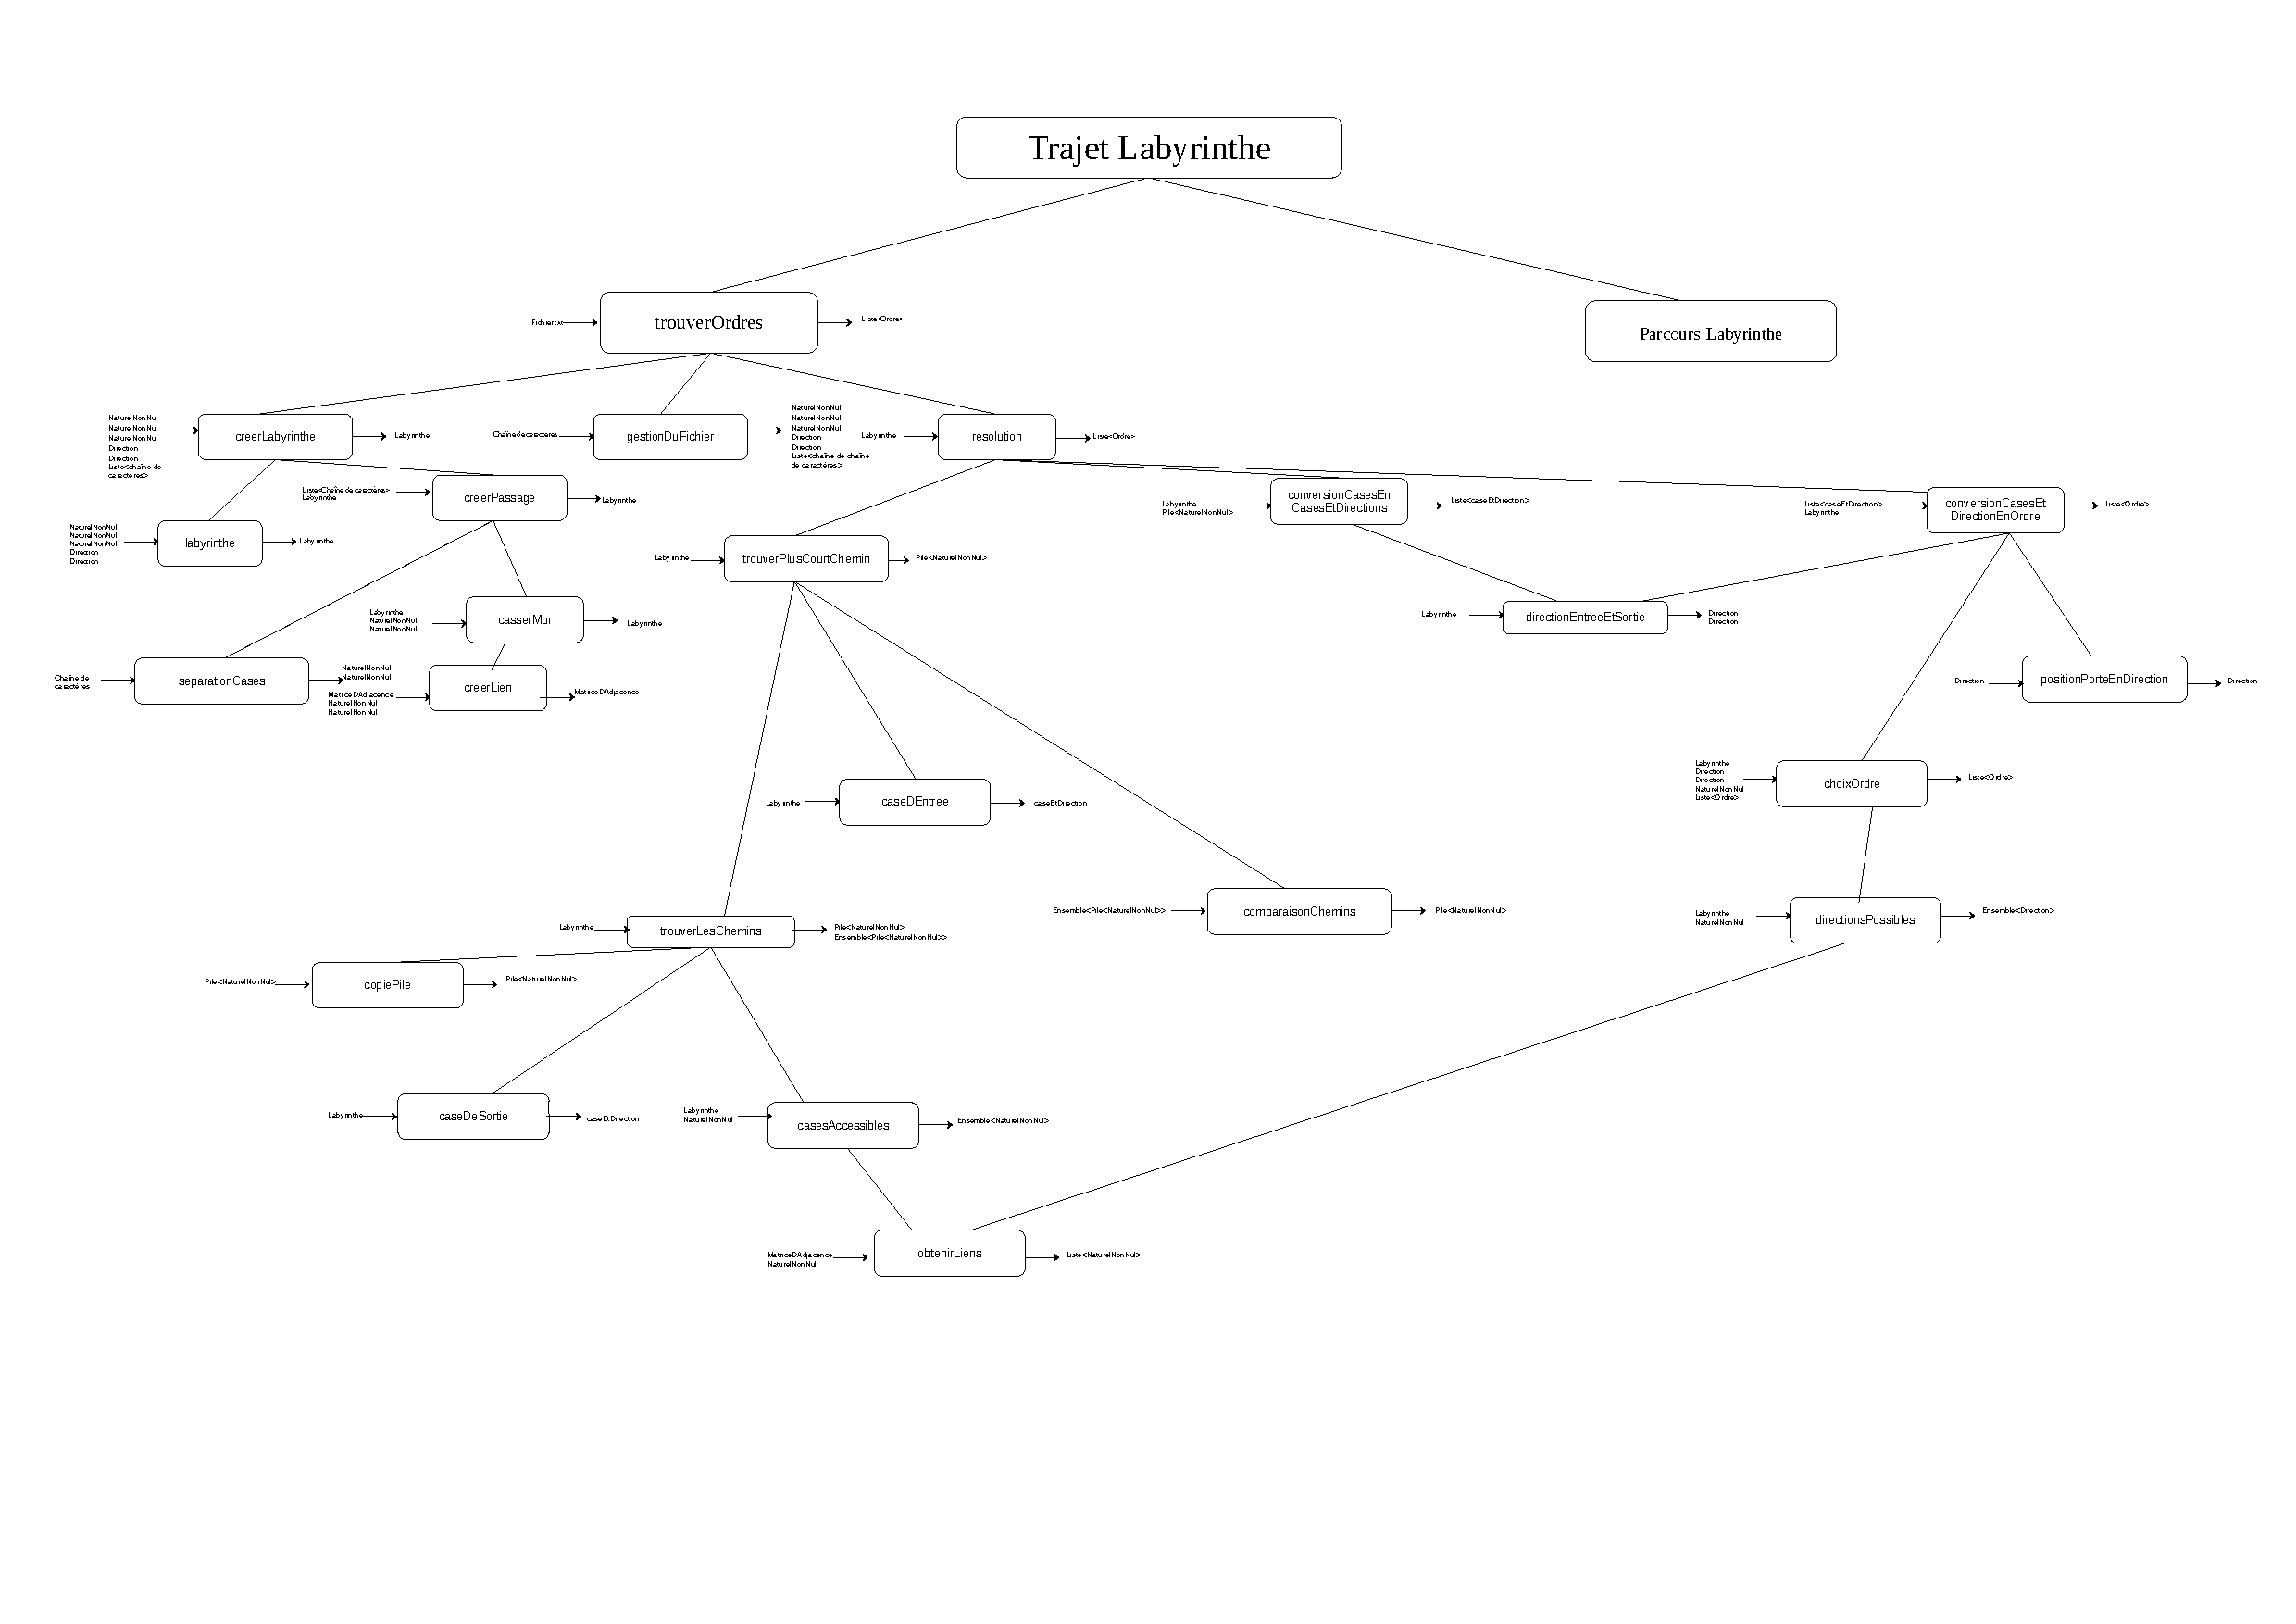
\includegraphics[width=1.2\textwidth]{algo/analyse/analyseDescendante_Algo.pdf} 
    \caption{Analyse descendante de la partie algorithmique}
    \label{fig:analyse}
\end{figure}


\begin{figure}[htbp]
    \centering
    \caption{Analyse descendante de la partie électronique} 
    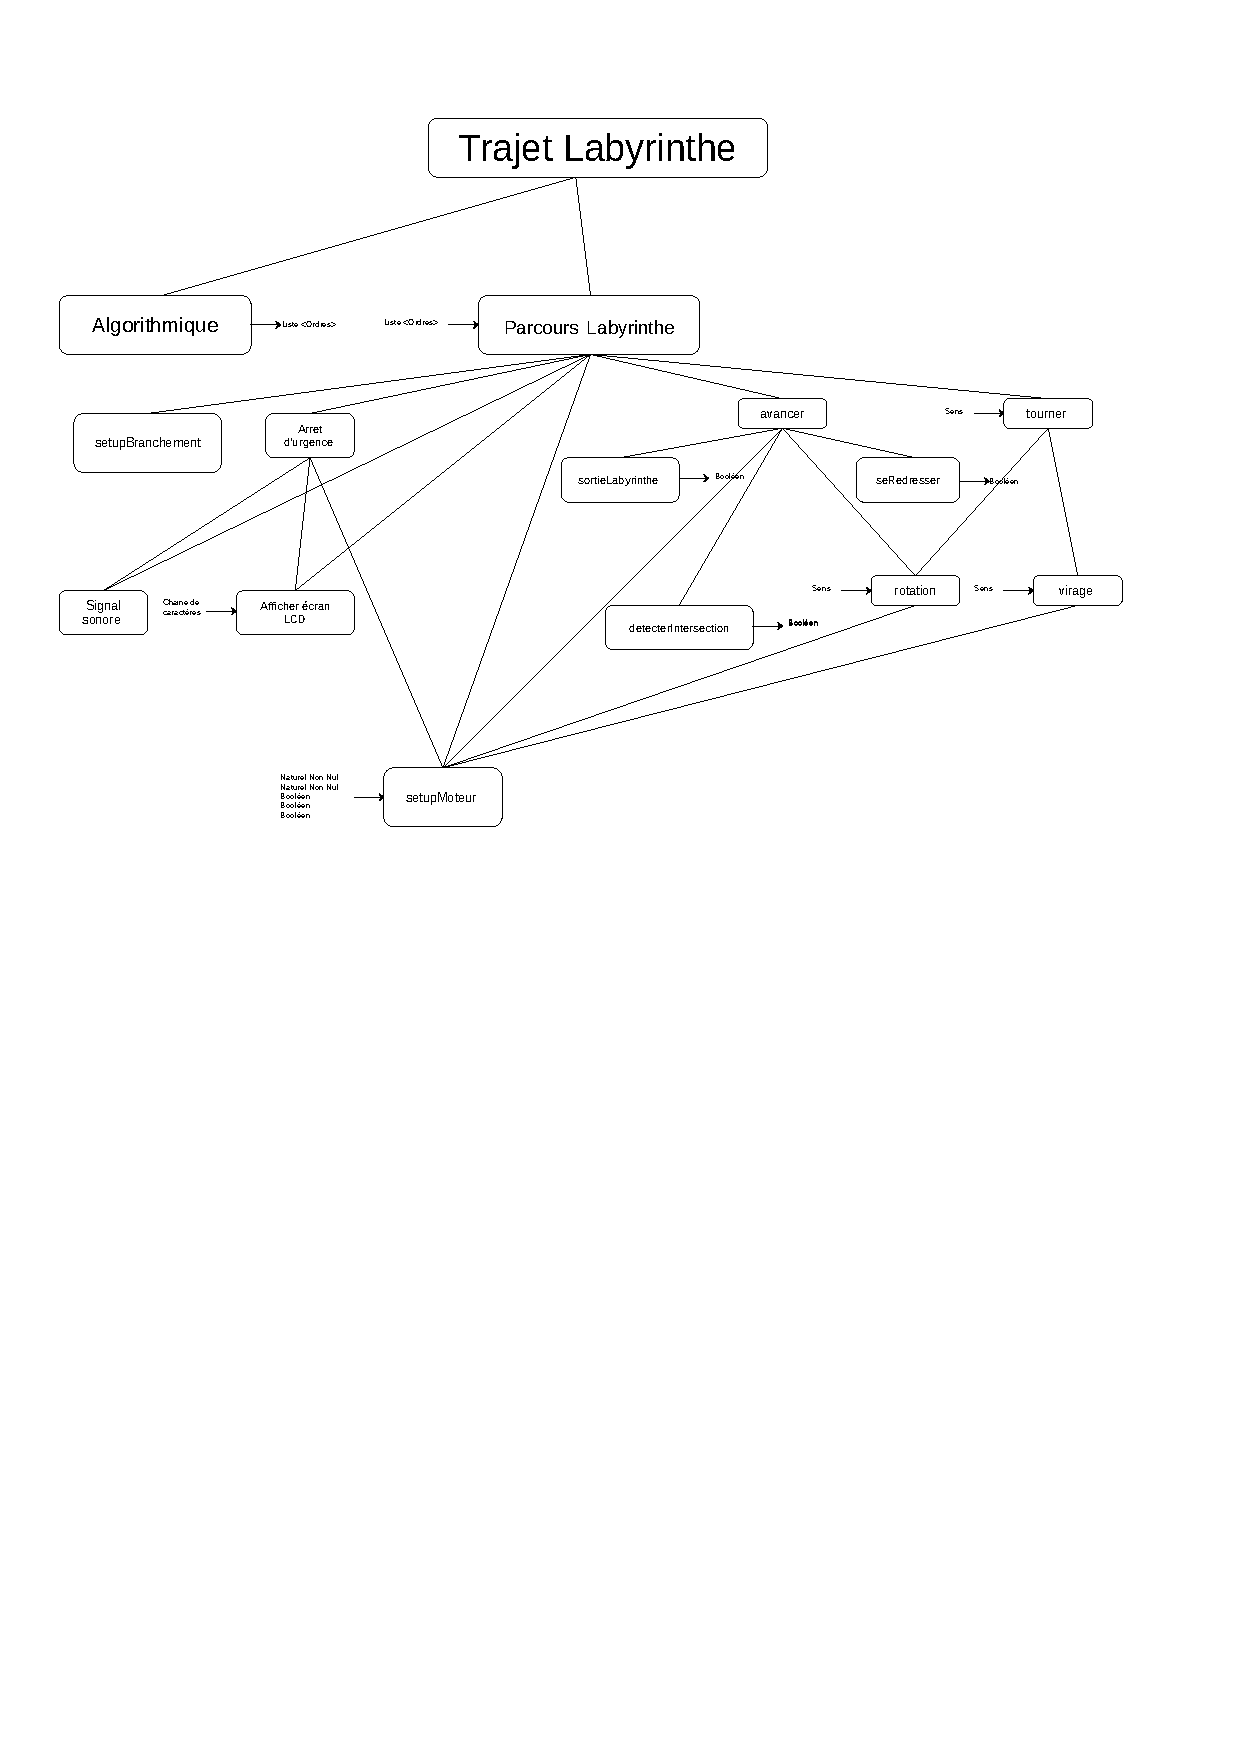
\includegraphics[width=1.2\textwidth]{elec/analyseDescendante_Elec.pdf}  
    \label{fig:analyse}
\end{figure}

\chapter{Conception préliminaire}

\setlength{\parskip}{0.05cm}

Cette partie répertorie les signatures des principaux algorithmes nécessaires à la résolution du problème du labyrinthe.
\vspace{0.5mm}

% CREER LABYRINTHE
\begin{algorithme}
    \signaturefonction
        {creerLabyrinthe}
        {caseDEntree : {\naturelNonNul}, \\ 
         caseDeSortie : {\naturelNonNul}, \\ 
         largeurLabyrinthe : {\naturelNonNul}, \\ 
         directionPorteEntree : {\direction}, directionPorteSortie : {\direction}, \\ 
         liaisonsCases : liste<{\cdc}>}
        {\Labyrinthe}
\end{algorithme}

\begin{algorithme}
    \signaturefonction
        {labyrinthe}
        {longueur : {\naturelNonNul}, \\ 
         caseDeDepart : {\naturelNonNul}, \\ 
         caseDeFin : {\naturelNonNul}, \\ 
         direction1 : {\direction}, direction2 : {\direction}}
        {\Labyrinthe}
    \remarque{
        Préconditions : \\
        caseDeDepart différent de caseDeFin : $caseDeDepart \neq caseDeFin$ \\[5pt]
        caseDeDepart appartient à: \\
        \quad $[|1, n|] \cup [|n^2 - n, n^2|] \cup \{k \in [|1, n|] \mid k \times n\} \cup \{k \in [|1, n|] \mid k \times n + 1\}$ \\[5pt]
        caseDeFin appartient à: \\
        \quad $[|1, n|] \cup [|n^2 - n, n^2|] \cup \{k \in [|1, n|] \mid k \times n\} \cup \{k \in [|1, n|] \mid k \times n + 1\}$.
    }
\end{algorithme}

\begin{algorithme}
    \signatureprocedure
        {creerPassage}
        {\paramEntreeSortie{Laby : {\Labyrinthe}}, \\ 
         \paramEntree{liaisonsCases : liste<{\cdc}>}}
\end{algorithme}

\begin{algorithme}
    \signatureprocedure
        {separationCases}
        {\paramEntree{casesASeparer : {\cdc}}, \\ 
         \paramSortie{case1 : {\naturelNonNul}, case2 : {\naturelNonNul}}}
\end{algorithme}

\begin{algorithme}
    \signatureprocedure
        {casserMur}
        {\paramEntreeSortie{Laby : {\Labyrinthe}}, \\ 
         \paramEntree{case1 : {\naturelNonNul}, case2 : {\naturelNonNul}}}
    \remarque{Préconditions:
    case1 $\neq$ case2, 
    case1 $\leq$ largeur(Laby)$^2$, 
    case2 $\leq$ largeur(Laby)$^2$.}
\end{algorithme}

\begin{algorithme}
    \signatureprocedure
        {creerLien}
        {\paramEntreeSortie{matrice : {MatriceDAdjacence}}, \\ 
         \paramSortie{nn1 : {\naturelNonNul}, nn2 : {\naturelNonNul}}}
\end{algorithme}

% GESTION DU FICHIER
\begin{algorithme}
    \signatureprocedure
        {gestionDuFichier}
        {\paramEntree{nomFichier : {\cdc}}, \paramEntreeSortie{listeLiaisons : liste<{\cdc}}, \paramSortie{largeur : {\nnn}, caseEntree : {\nnn}, caseSortie : {\nnn}, directionPorteEntree : {\direction}, directionPorteSortie : {\direction}}}  \\ 
\end{algorithme}

% RESOLUTION
\begin{algorithme}
    \signaturefonction
        {resolution}
        {Laby : {\Labyrinthe}}
        {liste<{ordre}>}
\end{algorithme}

% TROUVER PLUS COURT CHEMIN
\begin{algorithme}
    \signaturefonction
        {trouverPlusCourtChemin}
        {Laby : {\Labyrinthe}}
        {pile<{\naturelNonNul}>}
\end{algorithme}

\begin{algorithme}
    \signaturefonction
        {caseDEntree}
        {Laby : {\Labyrinthe}}
        {caseEtDirection}
\end{algorithme}

\begin{algorithme}
    \signatureprocedure
        {trouverLesChemins}
        {\paramEntree{laby : {\Labyrinthe}}, \\ 
         \paramEntreeSortie{cheminCourant : Pile<{\naturelNonNul}>, \\ 
         cheminsPossibles : Ensemble<Pile<{\naturelNonNul}>}}
\end{algorithme}		

\begin{algorithme}
    \signaturefonction
        {copiePile}
        {pile : Pile<{\naturelNonNul}>}
        {Pile<{\naturelNonNul}>}
\end{algorithme}

\begin{algorithme}
    \signaturefonction
        {caseDeSortie}
        {Laby : {\Labyrinthe}}
        {caseEtDirection}
\end{algorithme}

\begin{algorithme}
    \signaturefonction
        {casesAccessibles}
        {uneCase : {\naturelNonNul}, \\ 
         Laby : {\Labyrinthe}}
        {lesVoisins : Ensemble<{\naturelNonNul}>}
        \remarque{Préconditions:
    uneCase $\leq$ largeur(Laby)$^2$}
\end{algorithme}

\begin{algorithme}
    \signaturefonction
        {obtenirLiens}
        {uneCase : {\naturelNonNul}, \\ 
         matrice : {MatriceDAdjacence}}
        {lesVoisins : Liste<{\naturelNonNul}>}
\end{algorithme}

\begin{algorithme}
    \signaturefonction
        {comparaisonChemins}
        {cheminsPossibles : Ensemble<Pile<{\naturelNonNul}> >}
        {Pile<{\naturelNonNul}>}
\end{algorithme}

% CONVERSION CASES EN CASES ET DIRECTIONS
\begin{algorithme}
    \signaturefonction
        {conversionCasesEnCasesEtDirections}
        {Laby : {\Labyrinthe}, \\ 
         p : Pile<{\naturelNonNul}>}
        {liste<{caseEtDirection}}
\end{algorithme}

\begin{algorithme}
    \signaturefonction
        {directionEntreeEtSortie}
        {Laby : {\Labyrinthe}}
        {\direction, \direction}
\end{algorithme}

% CONVERSION CASES ET DIRECTIONS EN ORDRE
\begin{algorithme}
    \signaturefonction
        {conversionCasesEtDirectionsEnOrdres}
        {Laby : {\Labyrinthe}, \\ 
         casesDirections: liste<{caseEtDirection}}
        {liste<{ordres}}
\end{algorithme}

\begin{algorithme}
    \signaturefonction
        {directionEntreeEtSortie}
        {Laby : {\Labyrinthe}}
        {\direction, \direction}
\end{algorithme}

\begin{algorithme}
    \signaturefonction
        {choixOrdre}
        {Laby : {\Labyrinthe}, \\ 
         directionCasePrecedente : {\direction}, directionCaseActuelle : {\direction}, \\ 
         caseActuelle : {\naturelNonNul}, \\ 
         ordres : liste<{ordre}>}
        {\direction, \direction}
\end{algorithme}

\begin{algorithme}
    \signaturefonction
        {directionsPossibles}
        {Laby : {\Labyrinthe}, \\ 
         nnn : {\naturelNonNul}}
        {Ensemble<{\direction}>}
\end{algorithme}

\begin{algorithme}
    \signaturefonction
        {positionPorteEnDirection}
        {d : {\direction}}
        {\direction}
\end{algorithme}

% AUTRE 
\begin{algorithme}
    \signatureprocedure
        {afficherListeOrdre}
        {\paramEntree{ordres: liste<{ordre}}}
\end{algorithme}

\chapter{Conception détaillée}

    \lstset{
        language=C,
        basicstyle=\ttfamily\footnotesize,
        keywordstyle=\color{blue}\bfseries,
        commentstyle=\color{gray},
        stringstyle=\color{red},
        numbers=left,
        numberstyle=\tiny\color{gray},
        breaklines=true,
        frame=single,
        extendedchars=true, 
        literate={é}{{\'e}}1 {è}{{\`e}}1 {ê}{{\^e}}1 {à}{{\`a}}1 {ç}{{\c{c}}}1, 
        captionpos=b
    }

    Le groupe s'est concerté pour se fixer des contraintes de codage afin de faciliter la relecture du code par d'autres membres du groupe (tabulation, positionnement des parenthèses et accolades...). De plus, la conception détaillée nous permet de nous guider pour la phase d'écriture des algorithmes en C.
    \vspace{0.5mm}

    \section{Principes de développement}
        \subsection{Structure de l'algorithme}
            Pour implémenter l'algorithme nous avons décidé d'utiliser de nombreux types : listes, listes chaînées, ensembles ... afin d'avoir peu de fonctions à implémenter ensuite pour résoudre le problème du labyrinthe. De plus, l'ensemble de ces types permet une implémentation plus structurée, plus claire et plus évidente de par l'utilisation de fonctions et donc la création d'algorithmes plutôt courts, car de nombreuses opérations sont définies dans les types utilisées.

        \subsection{Les espaces de nommage}
            Les espaces de nommages sont primordiales lors de l'écriture collaborative d'algorithmes afin de garder un code clair et harmonieux. Alors, nous avons définis les conventions suivantes : 

            \begin{itemize}
                    \item Chaque type commence par une lettre majuscule, avec chaque nouveau mot également en majuscule. Exemple : \texttt{ListeDOrdre}. Chaque type est préfixé par ses initiales. Exemple : \texttt{LDO\_ListeDOrdre}.
                    \item Les fonctions et procédures sont toujours préfixées par le type qu'elles manipulent. Elles commencent toutes par une minuscule, avec chaque nouveau mot en majuscule. Exemple : \texttt{LAB\_initialisationLabyrinthe}.
                    \item Les variables sont toujours écrites en minuscules, avec une majuscule pour chaque nouveau mot. Exemple : \texttt{positionActuelle}.
                    \item L'ouverture d'une accolade se fait sur la même ligne que l'instruction dont elle dépend, et la fermeture de l'accolade est sur une nouvelle ligne.
                    \item Une indentation est ajoutée à chaque entrée dans une boucle ou une condition.
            \end{itemize}



    \section{Conception détaillée des fonctions principales}
        Ci-dessous sont répertoriées les principales signatures des algorithmes permettant de résoudre le labyrinthe.
        \vspace{0.2mm}
        \subsection{analyse Fichier}
            \begin{algorithme}
    \fonction{analyseFichier}{fichier : fichier.txt}{\nnn,\nnn,\\
    \nnn,Liste<ChaineDeCaracteres>}
        {taille : \nnn, entree : \nnn,\\
        sortie : \nnn, passages : Liste<ChaineDeCaracteres>}
        {
           \affecter{taille}{LireLigne(fichier)}
           \affecter{entree}{LireLigne(fichier)}
           \affecter{sortie}{LireLigne(fichier)}
           \tantque{non{fichier.estFinDeFichier()}}{
           	\instruction{Liste.inserer(passages,LireLigne(fichier))}
           }
           \retourner{taille, entree, sortie, passages}
        }
\end{algorithme}
 
        \subsection{Cases est presente dans pile}
            \begin{algorithme}
    \fonction{CasesEstPresenteDansPile}
    {pileCase : {Pile<noeud>}, pile : {Pile<noeud>}}
    {\booleen}
    {estPresent : \booleen , pileCaseTemp : {Pile<noeud>} , \\pileTemp : {Pile<noeud>}}
    {
        \affecter{estPresent}{Faux}
        \tantque{non estVide(pile) ou (estPresent = Vrai)}
            {
                \sialorssinon{obtenirElement(pile) = obtenirElement(pileCase)}
                    {   
                        \affecter{pileCaseTemp}{CopiePile(pileCase)}
                        \affecter{pileTemp}{CopiePile(pile)}
                        
                        \tantque{non estVide(pileCaseTemp) et \\(obtenirElement(pileTemp) = obtenirElement(pileCaseTemp))}
                            {
                                \instruction{dépiler(pileTemp)}
                                \instruction{dépiler(pileCaseTemp)}
                            }
                        \sialors{estVide(pileCaseTemp)}
                            {
                                \affecter{estPresent}{Vrai}
                            }                     
                    }
                    {
                        \instruction{dépiler(pile)}
                    }
            }
        \retourner{estPresent}
    }         
\end{algorithme}

 
        \subsection{Comparaison chemins}
            \newcommand{\pourDans}[2]{\textbf{pour} #1 \textbf{dans} #2 \textbf{faire}}

\begin{algorithme}
    \fonction{ComparaisonChemins}
        {lesPiles : Ensemble<Pile<noeud>>}
        {Pile<noeud>}
        {PlusCourtCheminDeSortie : \naturel , \\pileDuPlusCourtChemin : Pile<noeud>}
        {   
            \affecter{PlusCourtCheminDeSortie}{1000}
            \affecter{pileDuPlusCourtChemin}{Pile()}
            
            \pourDans{pile}{lesPiles}
                {
                    \affecter{longeurDeLaPile}{longueur(pile)}
                    
                    \sialors{longeurDeLaPile $<$ PlusCourtCheminDeSortie}
                        {
                            \affecter{PlusCourtCheminDeSortie}{longeurDeLaPile}
                            \affecter{pileDuPlusCourtChemin}{pile}
                        }
                }
            \retourner {pileDuPlusCourtChemin}
        }           

\end{algorithme}
 
        \subsection{conversion cases en cases et directions}
            \begin{algorithme}
	\fonction{conversionCasesEnCasesEtDirections}
  	{laby : Labyrinthe, p : Pile<\nnn>}
  	{Liste<caseEtDirection>}
  	{casesDirections : Liste<caseEtDirection>, \\
	caseActuelle, casePrecedente : \nnn, \\
	porteEntree, porteSortie : Direction}
	{
	\affecter{caseActuelle}{obtenirElement(p)} \\
	\affecter{casesDirections}{listeVide()} \\
	\instruction{directionEntreeEtSortie(laby, porteEntree, porteSortie)} \\
	\instruction{inserer(casesDirections, caseEtDirection(caseActuelle, positionPorteEnDirection(porteSortie)), 1)} \\
	\instruction{depiler(p)} \\

	\tantque{non estVide(p)}{
		\affecter{casePrecedente}{obtenirElement(p)} \\
      
      
			\sialors{casePrecedente $<$ caseActuelle}{
				\sialors{casePrecedente + 1 = caseActuelle}{
					\instruction{inserer(casesDirections, caseEtDirection(casePrecedente, D), 1)}
        			}
				\instruction{inserer(casesDirections, caseEtDirection(casePrecedente, B), 1)}
			}
			{
        		\sialors{(casePrecedente - 1) = caseActuelle}{
          			\instruction{inserer(casesDirections, caseEtDirection(casePrecedente, G), 1)}
        		}
        		\instruction{inserer(casesDirections, caseEtDirection(casePrecedente, H), 1)}
      			}
      	
	\instruction{depiler(p)} \\
	\affecter{caseActuelle}{casePrecedente}
    	}
    	\retourner{casesDirections}
  	}
\end{algorithme}




 
        \subsection{conversion cases et directions en ordres}
            \begin{algorithme}
	\fonction{conversionCasesEtDirectionsEnOrdres}{laby : Labyrinthe, \\casesDirections : 		Liste<caseEtDirection>}{Liste<Ordre>}
	{ordres : Liste<Ordre>, directionCaseActuelle,\\
	directionCasePrecedente,\\
	porteEntree, porteSortie : Direction,\\
    	caseActuelle, iLecture, iEcriture : \naturelNonNul}{
    	
	\affecter{ordres}{listeVide()}
	\affecter{iEcriture}{1}
	\affecter{iLecture}{1}
	\instruction{inserer(ordres, AV, iEcriture)}
	\instruction{directionEntreeEtSortie(laby, porteEntree, porteSortie)}
	\affecter{directionCasePrecedente}{positionPorteEnDirection(porteEntree)}    
	\tantque{non estVide(casesDirections)}{
	
	\affecter{directionCaseActuelle}{obtenirDirection(obtenirElement(casesDirections, iLecture))}
	\affecter{caseActuelle}{obtenirCase(obtenirElement(casesDirections, iLecture))}
	\affecter{iLecture}{iLecture + 1}
	\instruction{choixOrdre(ordres, iEcriture, laby, directionCasePrecedente,\\ directionCaseActuelle, caseActuelle)}
	\affecter{directionCasePrecedente}{directionCaseActuelle}
	}
	\retourner{ordres}
	}
\end{algorithme}
 
        \subsection{choix ordre}
            \begin{algorithme}
\procedure{choixOrdre}
	{\paramEntreeSortie{ordres : Liste<Ordre>, iEcriture : \\\naturelNonNul}, 
   \paramEntree{l : \Labyrinthe, directionCasePrecedente, \\directionCaseActuelle : Direction, 
   caseActuelle : \naturelNonNul}}
  {o : Ordre, directionsPossibles : Ensemble<Direction>, \\
   d : Direction, estIntersection : \booleen}
  {
    \sialorssinon{directionCasePrecedente = directionCaseActuelle}{
      \affecter{directionsPossibles}{obtenirDirectionsPossibles(l, caseActuelle)} \\
      \affecter{estIntersection}{Faux} \\
      \pourChaque{d}{directionsPossibles}{
        \cas{directionCaseActuelle}{
          \casclausegenerale{H}{
            \sialors{non(d = H ou d = B)}{
              \affecter{estIntersection}{Vrai}
            }
          }
          \casclausegenerale{B}{
            \sialors{non(d = H ou d = B)}{
              \affecter{estIntersection}{Vrai}
            }
          }
          \casclausegenerale{G}{
            \sialors{non(d = G ou d = D)}{
              \affecter{estIntersection}{Vrai}
            }
          }
          \casclausegenerale{D}{
            \sialors{non(d = G ou d = D)}{
              \affecter{estIntersection}{Vrai}
            }
          }
        }
      }
      
      \sialors{estIntersection}{
        \instruction{inserer(ordres, AV, iEcriture)} \\
        \affecter{iEcriture}{iEcriture + 1}
      }
    }
    {
      \cas{directionCasePrecedente}{
        \casclausegenerale{H}{
          \sialorssinon{directionCaseActuelle = G}{
            \affecter{o}{TG}
          }
          {
            \affecter{o}{TD}
          }
        }
        \casclausegenerale{B}{
          \sialorssinon{directionCaseActuelle = D}{
            \affecter{o}{TG}
          }
          {
            \affecter{o}{TD}
          }
        }
        \casclausegenerale{G}{
          \sialorssinon{directionCaseActuelle = B}{
            \affecter{o}{TG}
          }
          {
            \affecter{o}{TD}
          }
        }
        \casclausegenerale{D}{
          \sialorssinon{directionCaseActuelle = H}{
            \affecter{o}{TG}
          }
          {
            \affecter{o}{TD}
          }
        }
      }
      \instruction{inserer(ordres, o, iEcriture)} \\
      \affecter{iEcriture}{iEcriture + 1} \\
      \instruction{inserer(ordres, AV, iEcriture)} \\
      \affecter{iEcriture}{iEcriture + 1}
    }
  }
\end{algorithme}




 
        \subsection{Copie pile}
            \begin{algorithme}
	\fonction{CopiePile}
	{pile : Pile<noeud>}
	{Pile<noeud>}
	{}
	{
        \affecter{pileCopie}{Pile()} 
        
        \tantque{non estVide(pile)}{
		
                \instruction{empiler(pileCopie , obtenirElement(pile))}
                \instruction{dépiler(pile)}
	}
	
        \retourner{pileCopie}
	}         
\end{algorithme}
 
        \subsection{creer passage}
            \begin{algorithme}
\procedure
    {creerPassage}
    {\paramEntreeSortie{laby : Labyrinthe} \paramEntree{case1, case2 : \naturelNonNul}}
    {}
    {
        \sialors{EstCaseAccessible(Laby, case1, case2)}
        {
            \instruction{casserMur(Laby, case1, case2)}
        }
    }
\end{algorithme}

 
        \subsection{Longueur}
            \begin{algorithme}
	\fonction{LongueurPile}
	{pile : Pile<noeud>}
	{\naturelNonNul}
	{longueurDeLaPile : \naturel}
	{   
        \affecter{longueurDeLaPile}{0} 
        
        \tantque{non estVide(pile)}
            {
                \affecter{longueurDeLaPile}{longueurDeLaPile + 1}
                \instruction{dépiler(pile)}
            }
        \retourner{longueurDeLaPile}
    }         
\end{algorithme}
 
        \subsection{plus court chemin}
            \begin{algorithme}
	\fonction{trouverPlusCourtChemin}{labyrinthe : Labyrinthe}{Pile<{\naturelNonNul}>}
        {cheminCourant : Pile<{\naturelNonNul}>, 
           premiereCase : \naturelNonNul, 
           cheminsPossibles : Ensemble<Pile<{\naturelNonNul}> >, 
           cheminLePlusCourt : Pile<{\naturelNonNul}>}
        {
           \affecter{cheminCourant}{pile()}
           \affecter{premiereCase}{caseEntree(labyrinthe)}
           \affecter{cheminCourant}{empiler(cheminCourant, premiereCase)}
           \affecter{cheminsPossibles}{ensemble()}
           \instruction {trouverlesChemins{labyrinthe, cheminCourant, cheminsPossibles}}
           \affecter{cheminLePlusCourt}{comparaisonChemins(cheminsPossibles)}
           
           \retourner{cheminLePlusCourt}
        }
\end{algorithme}
 
        \subsection{trouver les chemins}
            
\begin{algorithme}
	\procedure{trouverLesChemins}{
        \paramEntree{labyrinthe : Labyrinthe}, 
        \paramEntreeSortie{cheminCourant : Pile<{\naturelNonNul}>, 
        cheminsPossibles : Ensemble<Pile<{\\\naturelNonNul}> >}
        }
        {
           uneCase : \nnn
        }
        {
           \sialors{non(estVide(cheminCourant))}{
           
              \sialorssinon{obtenirElement(cheminCourant) = caseSortie(labyrinthe)}{
              
                 \instruction {ajouter(cheminsPossibles, cheminCourant)}
              }
              {
                 \pourChaque{uneCase}{casesAccessibles(obtenirElement(cheminCourant))}{
                 
                    \sialors{non(estPresent(cheminCourant, uneCase))}{
                    
                       \affecter{cheminCourant}{empiler(cheminCourant, uneCase)}
                       \instruction {trouverPlusCourtCheminR(labyrinthe, cheminCourant,\\ cheminsPossibles)}
                    }
                 }
              }
              \affecter{cheminCourant}{depiler(cheminCourant)}
           }
        }
\end{algorithme}

        \vspace{2mm}

    \section{Développement en langage C}

        \vspace{2mm}
        Dès lors que l'ensemble des éléments essentiels à la résolution du problème du labyrinthe ont été identifié, vient l'étape de l'implémentation en langage C. D'abord, il s'agit de créer les interfaces à l'aide des .h . Comme nous utilisons de nombreux types, il est préférable de présenter directement les .h et .c liés à la sortie du labyrinthe.
    \subsection{Les .h principaux}
        Ci dessous sont présentés les fichiers .h principaux.
        \lstinputlisting[language=C]{../Programme/include/Labyrinthe/trouverLesOrdres.h}
   	\lstinputlisting[language=C]{../Programme/include/Labyrinthe/traitementLabyrinthe.h}
    	\lstinputlisting[language=C]{../Programme/include/Labyrinthe/trouverChemin.h}
    	\lstinputlisting[language=C]{../Programme/include/Labyrinthe/casesEnOrdres.h}
    	\lstinputlisting[language=C]{../Programme/include/Labyrinthe/gestionFichier.h}
        \vspace{2mm}

    \subsection{Les .c principaux}
        Ci dessous sont présentés les .c des .h présentés ci-dessus. Veuillez trouver les .c des types en Annexe.
        \lstinputlisting[language=C]{../Programme/src/Labyrinthe/solution.c}
        \lstinputlisting[language=C]{../Programme/src/Labyrinthe/trouverLesOrdres.c}
        \lstinputlisting[language=C]{../Programme/src/Labyrinthe/traitementLabyrinthe.c}
        \lstinputlisting[language=C]{../Programme/src/Labyrinthe/trouverChemin.c}
        \lstinputlisting[language=C]{../Programme/src/Labyrinthe/casesEnOrdres.c}
        \lstinputlisting[language=C]{../Programme/src/Labyrinthe/gestionFichier.c}
        \lstinputlisting[language=C]{../Programme/src/Labyrinthe/initialisationLabyrinthe.c}
        \lstinputlisting[language=C]{../Programme/src/main.c}
        \vspace{2mm}

   \subsection{Les .c de la partie électronique}
        Ci-dessous sont présentés les .c associés au code du robot.
        \lstinputlisting[language=C]{../Programme/src/elec/buzz.c}
        \lstinputlisting[language=C]{../Programme/src/elec/capteurLigne.c}
        \lstinputlisting[language=C]{../Programme/src/elec/capteurObstacle.c}
        \lstinputlisting[language=C]{../Programme/src/elec/ecran.c}
        \lstinputlisting[language=C]{../Programme/src/elec/codeMoteur.c}
        \lstinputlisting[language=C]{../Programme/src/elec/parcoursLabyrinthe.c}
        \lstinputlisting[language=C]{../Programme/src/elec/setup.c}

    \section{Tests unitaires}

        \vspace{2mm}
        Une fois que toutes les fonctions et procédures sont créées, il faut les tester indépendamment afin de s'assurer de leur fiabilité. C'est une étape très importante, car elle permet de rendre les tests d'intégration bien plus fiables. En effet, si un problème survient lors des tests d'intégration, cela signifie que c'est une erreur d'algorithmie et non d'implémentation. Nous avons donc réalisés pas moins de 124 tests unitaires sur les types. 
    \section{Tests d'intégrations}
        Une fois que nous avions la garantie que toutes les fonctions/ procédures fonctionnaient correctement, nous avons commencé l'étape des tests d'intégration. Celle-ci consiste à mettre en lien chaque fonction et de vérifier que celles-ci nous retournent bien les résultats attendus. 
        \subsection{Partie algorithmique}
            Concernant la partie algorithmique, le but était de vérifier que les fonctions de la sortie du labyrinthe sont corrects. Pour cela, on donne le fichier du labyrinthe à notre programme puis on vérifie que chaque partie du programme donne le résultat attendu.
            Cela permet de voir et comprendre les erreurs du programme à chaque étape pour ainsi les corriger, notamment en utilisant l'outil de débuggage permettant de s'arrêter à divers moments de l'exécution.\\

            Le but était de pouvoir identifier et de résoudre les erreurs plus rapidement. Ces tests ont été très pertinents car ils ont permis de relever certaines incohérences et identifier des aspects qui ont été mal anticipés durant le projet. Pour illustrer, la copie des piles, des listes, ou des ensembles qui n'avaient pas été réalisés correctement. C'est pour cela qu'il a fallu ajouter des fonctions spécifiques afin de réaliser des deep copies. De plus, nous avons réalisé que nos algorithmes n'étaient pas toujours des plus évidents. Par exemple, l'utilisation d'une pile stockant le chemin courant ainsi qu'un ensemble de pile stockant tous les chemins possibles. Pour trouver le chemin le plus court, il a donc fallu implémenter une fonction qui compare ces chemins. Cependant, après réflexion, il aurait été préférable d'utiliser une liste de cases. Cela nous aurait offert de nombreux avantages :
            \vspace{0.1mm}
            \begin{itemize}
            \item L'implémentation du type EnsembleDePileDeNNN n'était plus nécessaire.
            \item L'implémentation du type PileDeNNN n'était plus nécessaire.
            \item La manipulation de la Liste est bien plus simple que la manipulation de la Pile.
            \item L'implémentation de la fonction de comparaison des chemins pouvait être évitée.
            \end{itemize}

            Pour conclure, l'algorithme fonctionne parfaitement mais nous avons perçu quelques axes d'améliorations si c'était à refaire.

            \vspace{2mm}

        \subsection{Partie électronique}
            Nous avons dû tester chaque composant de manière indépendante, afin de vérifier le bon fonctionnement du composant et de ses fonctions associées. Le test s'est déroulé en 2 parties: 
            \begin{itemize}
                \item Le test électrique : le composant était branché à une source d'alimentation, puis à l'aide d'un voltmètre, nous avons effectué des prises de tensions pour vérifier le bon fonctionnement.
                \item Le test du code C : en gardant le composant branché, on exécute un programme simple pour vérifier si la réponse du composant est bien celle attendue. 
            \end{itemize}
            Dès lors, nous avons exécuté notre code pour vérifier le bon comportement du composant. Finalement, nous avons regroupé ensemble toutes les fonctions pour créer un algorithme global dans l'objectif de faire sortir le robot du labyrinthe.\\

            Encore une fois, ces tests ont été très pertinents et nous ont permis de prendre conscience de nos erreurs. Dans un premier temps, nous avons réalisé que la stratégie utlisée pour guider le robot au sein du labyrinthe était théoriquement bonne, mais physiquement trop complexe à mettre en place. En effet, la longueur des cases ne nous permettait pas de tourner correctement. Nous avons donc dû trouver une autre approche pour résoudre le labyrinthe. La difficulté résidait alors dans le fait que nous ne pouvions pas changer la position des capteurs à cause de la contrainte de temps. Cependant, la façon dont nous avons implémenté nos fonctions nous permettait de les réutiliser assez facilement dans un autre contexte.\\

            % explication fonctionnement du robot après changements.
            Le positionnement du capteur arrière s'est donc révélé plutôt inutile, ce qui nous a forçé à implementer le code à l'aide de 3 capteurs seulement, une tâche plutôt complexe quand la majorité des groupes utilisent 4 capteurs voire 5. Lorsque nous détections un virage, nous avancions un peu de manière à ne plus le détecter, puis nous tournions jusqu'à ce que nous récupérions la ligne avec le capteur du milieu. Il est intéressant de noter que cette manière de prendre les virages respecte bien la consigne de suivre les lignes tout en veillant à ne franchir aucun mur, c'est à dire que le robot restait parfaitement dans les cases.\\

            Finalement, bien que nous ayons réussi à trouver une méthode satisfaisante, nous avons rencontré quelques problèmes, notamment au niveau des intersections. Bien que nous sommes parvenus, à faire sortir le robot du labyrinthe proposé dans le sujet, en effectuant la résolution du labyrinthe à l'envers (la case d'entrée devient la case de sortie et vice-versa) nous nous sommes heurtés au problème suivant: le robot considère les successions d'ordres avancer comme un seul ordre avancer. En effet, bien qu'il reçoive les ordres d'avancer les uns à la suite des autres et bien qu'il soit censé poursuivre en ligne droite, le robot tourne. Le problème réside alors dans une entrée de boucle qui n'est pas respectée. Plus précisemment, lorsque le robot détecte une intersection, nous voulons qu'il continue jusqu'à ce qu'il ne la détecte plus, puis qu'il effectue l'ordre suivant. Cependant, celui ci n'attend pas de sortir de l'intersection et enchaine les ordres avancer très rapidement.\\ 

            Ainsi, lors de la soutenance, notre robot a parfaitement démarré en effectuant les quatre virages de suite, et a finalement rencontré le même problème. Nous sommes tout de même fiers du travail accompli.

  
\input{algo/codeC.tex}                

% Conclusion
\chapter{Conclusion}

\section{Conclusion globale sur le projet}
De manière plus générale, ce projet nous a permis d'assimiler et de renforcer de nombreuses compétences. En effet, celui-ci utilise un large pannel d'outils et de méthodes de travail indispensable pour un ingénieur. Bien que cette première expérience n'aie pas toujours été parfaitement réalisée, elle aura été très enrichissante. Elle nous aura permis de nous projeter plus concrètement sur le travail que nous aurons à effectuer, et les difficultés que nous rencontrerons, dans les années à venir.

\section{Ressenti personnel de chaque membre \\ du projet}

\begin{itemize}
    \item \textbf{Delaplace Yohann}\\ Le projet m'a permis de lier la théorie et la pratique en la mettant en œuvre sur le robot. Cela m'a aussi permis de m'habituer à utiliser Git afin de réaliser un travail en groupe. J'ai eu l'occasion de programmer en C et en Shell, ce qui m'a permis de comprendre plus en profondeur les notions abordées en cours. Concernant le groupe de travail, chacun avait sa tâche assignée par le chef de projet, avec la date limite à ne pas dépasser pour que le projet puisse bien avancer, et chacun d'entre nous a respecté ce fonctionnement, permettant au projet de se développer plus rapidement. De plus, je tiens à souligner la bonne entente dans notre groupe de travail, ce qui nous a permis de rester motivés du début à la fin et de tout donner pour réussir et avoir un projet qui fonctionne. Je pense que si ce projet a pu être mené à bien, c'est grâce au grand investissement personnel de chacun.
\end{itemize}
\vspace{5mm}

\begin{itemize}
    \item \textbf{Lenoble Louis}\\Bien que le robot ne soit pas encore totalement opérationnel, je suis fier du chemin parcouru par le groupe et de la manière dont chacun a su trouver sa place. Cette complémentarité a créé une dynamique positive et productive, où les idées de chacun enrichissaient le projet. J’ai particulièrement apprécié l’engagement collectif et l’entraide qui se sont développés au fil des séances.\\

Ensuite, ce projet a profondément changé ma manière de percevoir le travail en groupe. J'ai appris à mieux écouter, à anticiper les besoins des autres et à m'adapter aux imprévus. De plus, j'ai pris conscience que l'organisation rigoureuse et la communication ouverte ont été d'une très grande importance pour garantir un avancement régulier et efficace. C’est un apprentissage que je considère précieux, et je me sens désormais bien mieux préparé pour travailler de manière collaborative dans d'autres contextes.\\

Enfin, en tant que chef de projet, cette expérience a été révélatrice. Je me suis rendu compte que ce rôle demande bien plus qu'une simple coordination : il s'agit d'être à l'écoute, de motiver, et de savoir tirer le meilleur de chaque membre du groupe. Organiser les séances, planifier les objectifs et faire des bilans réguliers m'ont demandé beaucoup de temps, mais cela m’a permis de développer une meilleure capacité d’analyse et de décision. Cette immersion dans la gestion de projet m’a permis de grandir, à la fois en tant que leader et en tant qu’individu capable de travailler de façon autonome.
\end{itemize}
\vspace{5mm}

\begin{itemize}
    \item \textbf{Planchot Maël}\\
Ce projet a été une expérience riche et très enrichissante, tant sur le plan technique que personnel. La diversité des tâches à accomplir, ainsi que les imprévus rencontrés, ont mis à l'épreuve notre capacité d'adaptation et notre gestion du stress. Bien que le produit final ait encore des points perfectibles, les résultats obtenus sont encourageants, et je suis satisfait des solutions que nous avons pu apporter. Ce projet m’a permis de me perfectionner en c, de mieux abordés les problèmes de débeugage et d'améliorer ma communication au sein d'une équipe.
\end{itemize}
\vspace{5mm}

\begin{itemize}
    \item \textbf{Sanson Dylan}\\Ce projet a été une expérience à la fois stimulante et formatrice. La complexité des tâches, combinée à la gestion du temps, a été un véritable défi. En tant qu’équipe, nous avons dû nous adapter rapidement, mais la répartition des rôles et l’entraide ont permis de maintenir une bonne dynamique. J’ai particulièrement apprécié de pouvoir mettre en pratique les concepts appris en cours, notamment en programmation C. Bien que le robot ne soit pas totalement fonctionnel, nous avons fait de réels progrès, et je suis fier du travail accompli. Ce projet m’a permis de développer de nouvelles compétences techniques et humaines, en particulier dans le travail en équipe et la gestion de projet.
\end{itemize}
\vspace{5mm}

\begin{itemize}
    \item \textbf{Sourdrille Nathan}\\
    Ce projet était une première grande expérience pour moi de part la quantité de travail à fournir, l'étendu de la durée du projet, l'utilisation de nouveaux outils et le travail en groupe de cinq. D'abord, la quantité de travail à fournir était très importante, et cela bien que nous ayons réparti, il me semble, plutôt bien le travail. Ce projet s'est étendu sur deux mois mais quelques jours de plus aurait été grandement apprécié, afin de résoudre les problèmes rencontrés lors de la phase de test, que nous n'avons pu effectuer que durant la dernière semaine. D'autre part, je n'avais jamais utilisé, hormis leur introduction durant les séances de td, les outils gitlab, latex ... C'était aussi une première expérience de vrai programmation en C. Cependant c'était très intéressant d'exploiter ce que nous avons pu voir dans les différentes matières, et de pousser plus loin la SE par exemple, en naviguant dans le terminal, créant des scripts bash ... Globalement, le projet est très intéressant et très satisfaisant quand on arrive finalement à faire sortir le robot du labyrinthe, cependant il demande énormément de travail personnel, de l'organisation et une entente harmonieuse entre les membres du groupe est indispensable pour mener le projet à son terme.
\end{itemize}





 

% Annexe
\chapter{Annexes}

\lstset{ 
    basicstyle=\ttfamily\small,
    breaklines=true, 
    frame=single, 
    xleftmargin=20pt,
    xrightmargin=20pt, 
}

\section{Références bibliographiques}


    \begin{itemize}
        \item $\bullet$ \url{https://cdn.bodanius.com/media/1/a9c1593_fiche-technique-du-tcrt5000.pdf} pour les capteurs de positions 
        \item $\bullet$ \url{https://www.adeept.com/ultrasonic-sr04_p0047.html} pour le capteur a ultrason (récupération de la tension et du courant d'entrée necessaire pour déterminer la puissance)
        \item $\bullet$ \url{https://cdn.bodanius.com/media/1/8c2164078_l293d.pdf} pour les bouclier thermiques (carte moteur)
        \item $\bullet$ \url{https://www.openhacks.com/uploadsproductos/eone-1602a1.pdf} pour l'écran LCD et le controleur de l'écran (référence dans le tableau section: 3.0ELECTRICAL CHARACTERISTICS)
        \item $\bullet$ \url{https://moodle.insa-rouen.fr/pluginfile.php/184607/mod_resource/content/5/Lab_Sheet__1.pdf} pour la LED suivis de 
        \item $\bullet$ \url{https://www.adeept.com/4pcsled_p0104.html} pour la la LED (documentation et informations manquantes pour le sujet, on utilise donc le cas général pour une led rouge)
        \item $\bullet$ \url{https://www.adeept.com/passivebuzzer_p0284.html} pour le buzzer, la documentation est manquante, on prendra la cas "général" de la consomation énergétique d'un buzzer. 
        \item $\bullet$ \url{https://www.adeept.com/2xn20-with-holder_p0335.html} pour les moteurs, consommation maximale en ampère prise en compte.         
        \item $\bullet$ \url{https://moodle.insa-rouen.fr/pluginfile.php/31526/mod_label/intro/documentation.pdf} pour la documentation Latex
        
    \end{itemize}

\newpage
\section{Glossaire}
    \begin{table}[ht]
        \begin{adjustwidth}{-3cm}{-3cm}
            \centering
            \begin{tabular}{|p{1cm}|p{5cm}|p{10cm}|}
                \hline
                \textbf{Nom} & \textbf{abréviation} & \textbf{Définition}\\
                \hline
                TAD & Type Abstrait de Données & Structure de données définie par des opérations (est indépendant du language de programmation).\\
                \hline
                GPIO & General Purpose Input/Output & Une broche de la carte Raspberry qui peut être configurée comme une entée pour reçevoir un signal ou comme une sortie pour reçevoir un signal.\\ 
                \hline
                SDA & Serial Data Line & Ligne de commmunication utilisé dans les bus I2C utilisée pour envoyer et reçevoir des données.\\
                \hline
                SCL & Serial Clock Line & Ligne de communication utilisé dans les bus I2C utilisée pour synchoniser la transmition de données (définit l'orloge).\\
                \hline
                I2C & Inter-Integrated Circuit & Protocole de communication entre composants.\\
                \hline
                GND & Ground & Masse du circuit électronique.\\
                \hline
                VCC & Voltage at the Common Collector & Source de tension positive d'alimentation d'un circuit électronique.\\
                \hline
                Trig & Trigger & Ligne utilisée pour le signal de déclanchement d'un capteur.\\
                \hline
                Tx & Transmit & Ligne utilisée pour la transmition de données.\\
                \hline
                Rx & Receive & Ligne utilisée pour la réception de données.\\
                \hline
                Echo & écho & Signal reçu du capteur à ultrason après réverbération du son sur une surface.\\
                \hline
                LED & Light Emitting Diode & Composant électronique qui emmet de la lumière lorsque un certain seuil de tension est dépassé (consomme moins d'électricité qu'une lampe classique).\\
                \hline
                PWM & Pulse Width Modulation & Le signal envoyé peut changer la durée des impulsions. \\     
                \hline
                SD & Secure Digital & carte mémoire pour stocker des données. \\
                \hline
                SSH & Secure Shell & Protocole de communication crypté pour se connexter à distance sur un autre appareil.\\
                \hline
                RAM & Random Acces Memory & Mémoire en accès direct, stocke temporairement des données.\\
                \hline
                EN & Enable & Ligne utilisée pour activer ou désactiver un circuit électronique.\\
                \hline
                LCD & Liquid Crystal Display & Permet de crontrôler la quantité de lumière qui passe à travers de l'écran à l'aide d'un champ électrique.\\
                \hline
            \end{tabular}
        \end{adjustwidth}
    \end{table}


\section{Analyses descendente version PDF} 
    Ci dessous sont présentés en format page entière les analyses descendantes mises en place lors du cycle en V.
    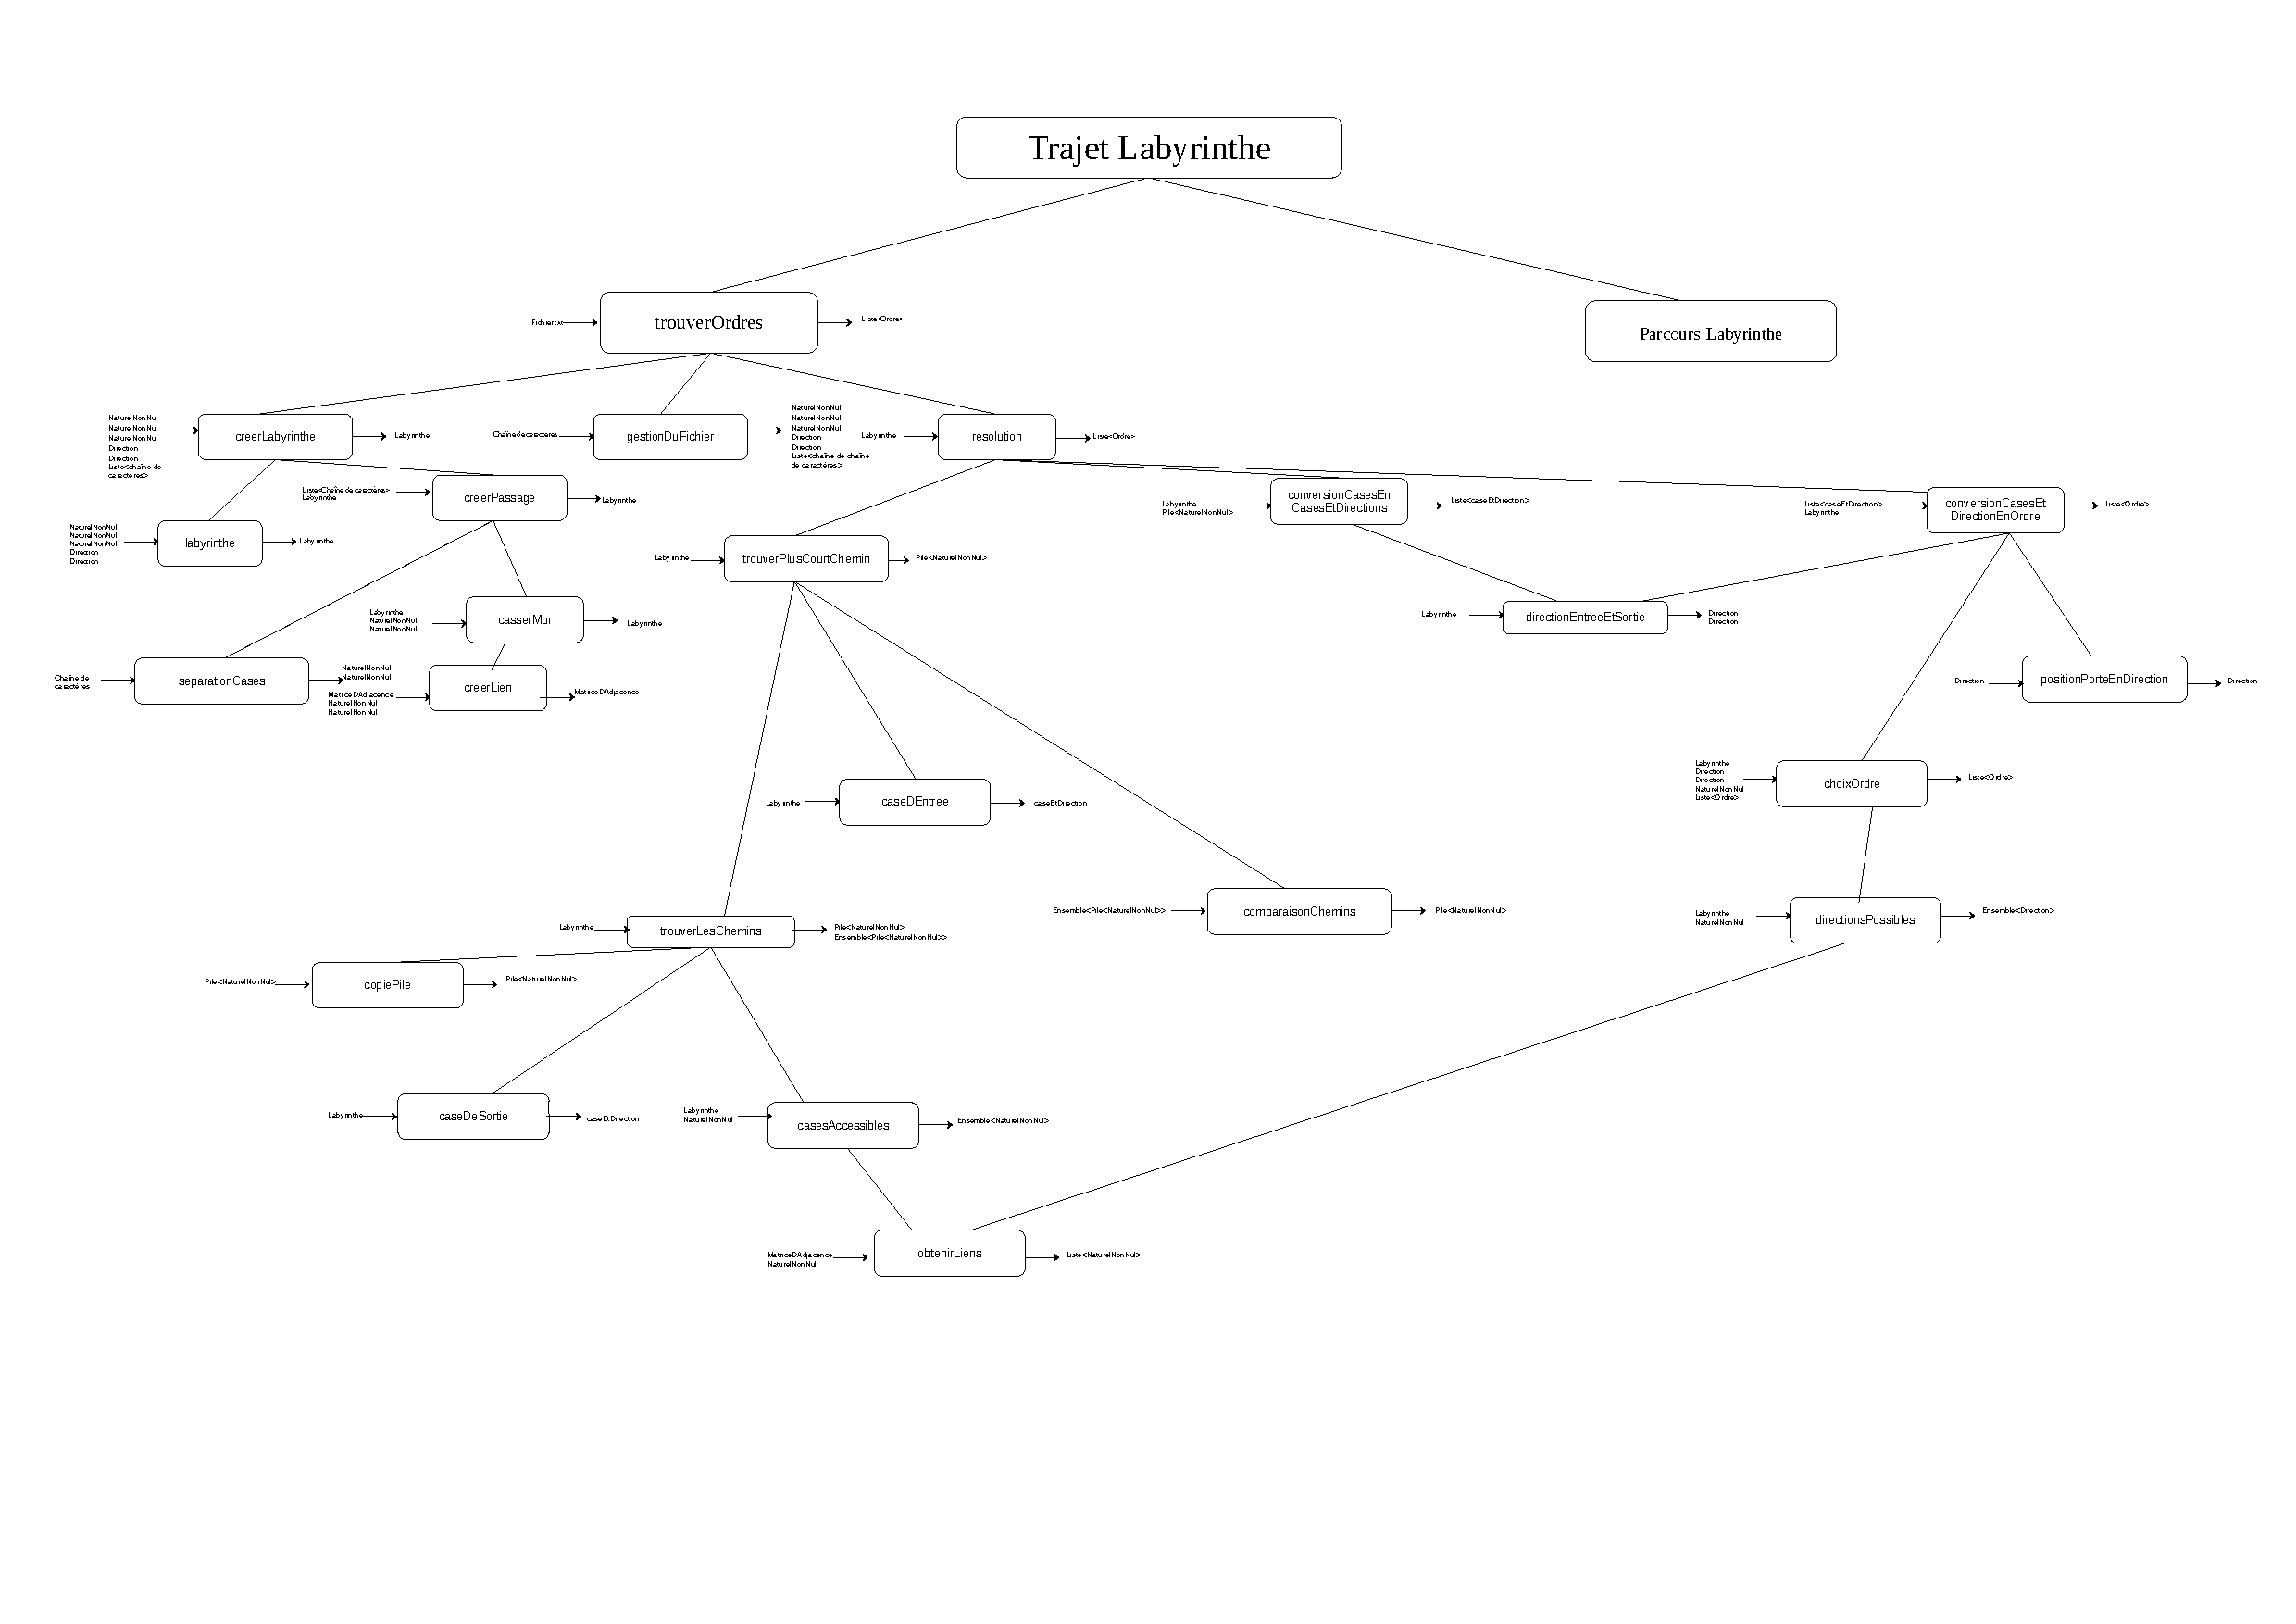
\includepdf[pages=-]{algo/analyse/analyseDescendante_Algo.pdf} 
    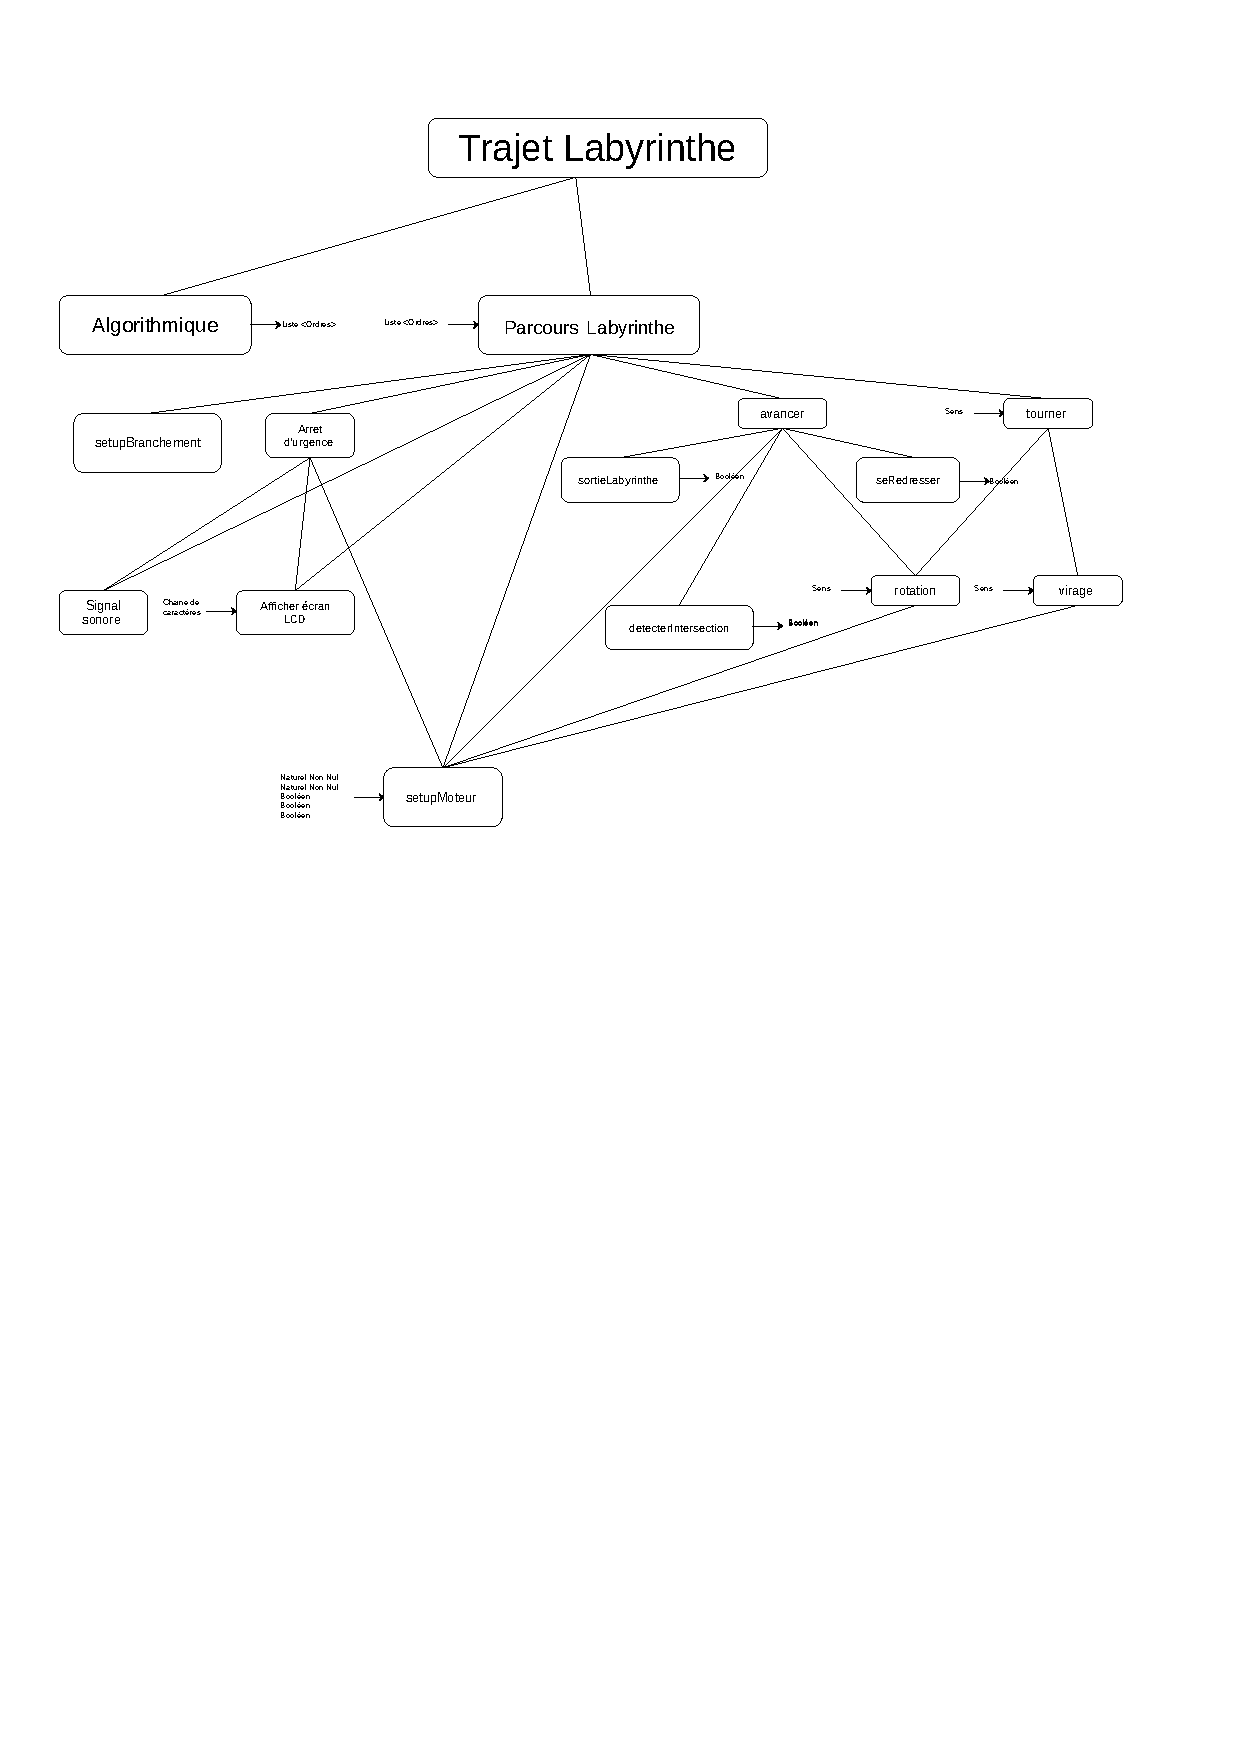
\includepdf[pages=-]{elec/analyseDescendante_Elec.pdf} 

\section{Fichiers .c}

    \subsection{Les Types}
        \subsubsection{Les listes}
            \lstinputlisting[language=C]{../Programme/src/Types/ListeDeNNN.c}
            \lstinputlisting[language=C]{../Programme/src/Types/ListeDOrdre.c}
            \lstinputlisting[language=C]{../Programme/src/Types/ListeDeCDC.c}
            \lstinputlisting[language=C]{../Programme/src/Types/ListeDeCaseEtDirection.c}

        \subsubsection{Les listes chaînées}
            \lstinputlisting[language=C]{../Programme/src/Types/ListeChaineeDeNNN.c}
            \lstinputlisting[language=C]{../Programme/src/Types/ListeChaineeDOrdre.c}
            \lstinputlisting[language=C]{../Programme/src/Types/ListeChaineeDeCDC.c}
            \lstinputlisting[language=C]{../Programme/src/Types/ListeChaineeDeCaseEtDirection.c}
            \lstinputlisting[language=C]{../Programme/src/Types/ListeChaineeDeDirection.c}
            \lstinputlisting[language=C]{../Programme/src/Types/ListeChaineeDePileDeNNN.c}

        \subsubsection{Les ensembles}
            \lstinputlisting[language=C]{../Programme/src/Types/EnsembleDeNNN.c}
            \lstinputlisting[language=C]{../Programme/src/Types/EnsembleDeDirection.c}
            \lstinputlisting[language=C]{../Programme/src/Types/EnsembleDePileDeNNN.c}

        \subsubsection{Les autres types}
            \lstinputlisting[language=C]{../Programme/src/Types/PileDeNNN.c}
            \lstinputlisting[language=C]{../Programme/src/Types/MatriceDAdjacence.c}
            \lstinputlisting[language=C]{../Programme/src/Types/Ordre.c}
            \lstinputlisting[language=C]{../Programme/src/Types/caseEtDirection.c}
            \lstinputlisting[language=C]{../Programme/src/Types/Direction.c}
            \lstinputlisting[language=C]{../Programme/src/Types/labyrinthe.c}





\end{document}

